\documentclass[
    a4paper,            % DIN A4
    DIV=10,             % Schriftgröße und Satzspiegel
    oneside,            % einseitiger Druck
    BCOR=5mm,           % Bindungskorrektur
    parskip=half,       % Halber Abstand zwischen Absätzen
    numbers=noenddot,   % Kein Punkt hinter Kapitelnummern
    bibtotoc,           % Literaturverzeichnis im Inhaltsverzeichnis
    listof=totoc        % Abbildungs- und Tabellenverzeichnis im Inhaltsverzeichnis
]{scrreprt}
\usepackage{../style/thesisstyle}

%\makeglossaries           % create all glossary entries (remember: run makeglossaries manually)
%\loadglsentries{thesisglossaries.tex}  % load acronym, symbol and glossary entries

\sisetup{locale = DE}     % siunitx locale setup
%\DeclareSIUnit \fps{fps}  % a custom unit (usage: \SI{24}{\fps})

\usepackage{tikz}
\usepackage{pgfplots}
\newcommand{\code}{\texttt}

%\bibliographystyle{plain}
\bibliographystyle{alpha}

\begin{document}
    % !TEX root = ../thesis.tex
%
% configurations
%

% English Language support
% -> uncomment if needed
% Beta!
%\fullenglish{yes}
\fullenglish{no}

% text field
%-> replace supervisor names with correct ones
\firstSupervisor{Prof. Dr.-Ing. Jane Doe}
\secondSupervisor{Prof. Dr. John Doe}

% text field
%-> replace title with your thesis title
\thesisTitle{Das Leben, das Universum und der ganze Rest}
\thesisTitleEN{Life, the Universe and Everything}

% text field
%-> replace the key words with your own key words
\keywordsDE{Leben, Universum, Alles}
\keywordsEN{Life, Universe, Everything}

% text field
%-> replace the text with a description of the thesis
\abstractDE{Arthur Dents Reise in eine neue Zukunft \dots}
\abstractEN{Arthur Dents travel to a new future \dots}

% text field
%-> replace john with your name
\thesisAuthor{John Doe}

% text field
%-> enter the submission date
\submissionDate{07. Juni 1954}

% switch - uncomment only one
%-> uncomment NDA or public
%\NDA{yes}
\NDA{no}

% switch - uncomment only one
%-> uncomment old standard cover or cover Corporate Design 2017
\Cover{CD2017}
%\Cover{CD2017NoLogo}
%\Cover{Std2018}
%\Cover{Std2018_green} 			% with green bar

% switch - uncomment only one
%-> uncomment to show list of figures or not
\ListOfFigures{yes}
%\ListOfFigures{no}

% switch - uncomment only one
%-> uncomment to show list of tables or not
\ListOfTables{yes}
%\ListOfTables{no}

% switch - uncomment only one
%-> uncomment to show list of accronyms or not
\ListOfAccronyms{yes}
%\ListOfAccronyms{no}

% switch - uncomment only one
%-> uncomment to show list of symbols or not
\ListOfSymbols{yes}
%\ListOfSymbols{no}

% switch - uncomment only one
%-> uncomment to show list of glossary entries or not
\Glossary{yes}
%\Glossary{no}

% switch - uncomment only one
%-> uncomment the study course you are in
\studycourse{ITS}
%\studycourse{TI}
%\studycourse{AI}
%\studycourse{WI}
%\studycourse{EI}
%\studycourse{REE}
%\studycourse{BMP}		
%\studycourse{BMP-hp}	 % Internship Report in M&P
%\studycourse{BMT}
%\studycourse{BMT-st}    % Study / home assignment in BMT
%\studycourse{BMT-hp}    % Internship Report in BMT
%\studycourse{MI}
%\studycourse{MIK}
%\studycourse{MA}
    % load all settings

    \hyphenation{Ba-che-lor-the-sis Mas-ter-the-sis}

% Cover page here, no page number
    \ICoverPage

% PDF Metadata
    % !TEX root = ../thesis.tex
%
% PDF Metadata integration
% @author Thomas Lehmann
%

% PDF Metadata
\hypersetup{
pdftitle={\IthesisTitle},
pdfauthor={\IthesisAuthor},
pdfkeywords={\IkeyWordsEN}
}

% Titlepage is page one even if the number is not shown.
    \pagenumbering{roman}
% Title page here
    % !TEX root = ../thesis.tex
%
% title page
% @author Thomas Lehmann
% Hints for title page and page numbering: https://en.wikipedia.org/wiki/Title_page
%
\title{\IthesisTitle}   % set latex default title to be used by hyperref in pdf
\author{\IthesisAuthor} % set latex default author to be used by hyperref in pdf

\newpage
\thispagestyle{empty}
{\fontfamily{phv}\selectfont
  \hfuzz=20pt       % suppress warnings due to extension onto page margins

  % Author of thesis
  \vspace*{1cm}
  \begin{minipage}[b]{\textwidth}
    \fontsize{14pt}{20pt}
    \selectfont
    \begin{center}
      \IthesisAuthor
    \end{center}
  \end{minipage}

  % Title of thesis
  \vspace{1.5cm}
  \begin{minipage}[b][0cm][t]{\textwidth}
    \fontsize{18pt}{20pt}
    \selectfont
    \begin{center}
      \IthesisTitle
    \end{center}
  \end{minipage}

  % Important information
  \begin{textblock*}{\textwidth}(40mm,210mm)
    \begin{minipage}[b]{\textwidth}
      \hbadness=10001    % suppress underfull warning due to short text
      \fontfamily{cmr}\selectfont
      \fontsize{12pt}{14pt}
      \selectfont
      \ifdefined\ILanguageEN
        \IthesisKindEN ~submitted for examination in \IthesisExaminationEN \\
        in the study course \textit{\IstudyCourseName} \\
        at the \IthesisDepartmentFullEN \\
        at the \IthesisFacultyFullEN \\
        at University of Applied Science Hamburg\\

        Supervisor: \IfirstSv \\
        \ifdefined\IisTermPaper
          % left blank
        \else
          \ifdefined\IisInternshipReport
	  Supervised: \IsecondSv\\
          \else
        Supervisor: \IsecondSv \\
          \fi\fi
        
        Submitted on: \ISubDate \\
      \else
      	\ifdefined\IisInternshipReport
        \IthesisKindDE ~eingereicht im Rahmen des \IthesisExaminationDE \\	
	\else
        \IthesisKindDE ~eingereicht im Rahmen der \IthesisExaminationDE \\
        \fi
	im Studiengang \textit{\IstudyCourseName} \\
        am \IthesisDepartmentFull \\
        der \IthesisFacultyFull \\
        der Hochschule für Angewandte Wissenschaften Hamburg\\

        Betreuender Prüfer: \IfirstSv \\
        \ifdefined\IisTermPaper
          % left blank
        \else
          \ifdefined\IisInternshipReport
        betriebliche Betreuung: \IsecondSv \\							
	  \else
        Zweitgutachter: \IsecondSv \\
        \fi\fi

        Eingereicht am: \ISubDate \\
      \fi
    \end{minipage}
  \end{textblock*}
}


% Abstract page here
    % !TEX root = ../thesis.tex
%
% abstract page
% @author Thomas Lehmann
%
\newpage
\thispagestyle{plain}
\clearpage
\hfuzz=12pt       % suppress warnings due to extenstion onto page margins

\ifdefined\ILanguageEN
  % just skip
\else
    \textbf{\IthesisAuthor}

    \vspace{0.3cm}
    \textbf{Thema der Arbeit}

    \IthesisTitle

    \vspace{0.3cm}
    \textbf{Stichworte}

    \IkeyWordsDE

    \vspace{0.3cm}
    \textbf{Kurzzusammenfassung}

    \begin{minipage}{\textwidth}
    \IabstractDE
    \end{minipage}
\fi

\vspace{1.0cm}
\textbf{\IthesisAuthor}

\vspace{0.3cm}
\textbf{Title of Thesis}

\IthesisTitleEN

\vspace{0.3cm}
\textbf{Keywords}

\begin{minipage}{\textwidth}
\IkeyWordsEN
\end{minipage}

\vspace{0.3cm}
\textbf{Abstract}

\IabstractEN


% Table of contents here
    \tableofcontents

% List of figures here
    \IListOfFigures

% List of tables here
    \IListOfTables

% List of accronyms here
    \IListOfAccronyms

% List of symbols here
    \IListOfSymbols

% Uncomment if list of source code is needed (rarely).
%\lstlistoflistings  % requires package listings, needs to uncommenting of usepackage

% path to the chapters folder is set to find the images used there
    \graphicspath{ {./chapters/.images} }


% Chapters
    \clearpage
    \pagenumbering{arabic}
    % introductory chapter
% @author Kalvin Döge
%
\chapter{Einleitung}\label{ch:einleitung}

Mit dem Klimawandel wird es immer deutlicher, dass der Verzicht auf ein Pkw und der Wechsel auf den öffentlichen Personennahverkehr oder das Fahrrad eine nachhaltigere Wahl darstellt.
Doch leider ist es nicht ganz so einfach: Gerade in der Großstadt Hamburg gehört Stau tagsüber quasi zum Alltag auf den Straßen.
Pkws, Lkws und Fahrradfahrer teilen sich auf manchen Wegen immer wieder dieselbe Spur und halten auch an derselben Ampel, wenn wieder keine Fahrradspur gerade zur Verfügung steht.
Doch die Stadt Hamburg fängt an, das Fahrrad in dem Verkehr in manchen Stadtvierteln zu bevorzugen und die Lichtsignalschaltungen nach ihnen auszurichten~\cite{NDR2022}.
So auch gegen das Ende letzten Jahres: Im Stadtteil Eimsbüttel sollen Fahrradfahrern und Fußgängern dem Autoverkehr bevorzugt werden, indem eine Ampel an einer stark befahrenen Überquerung vor anderen vorlassen.

Auch wenn dies nur ein Anfang ist, so lässt sich daraus die Frage ableiten: Ließen sich Lichtsignalschaltungen so zeitlich einstellen, dass sie einem Fahrradfahrer den gesamten Weg eine ,,Grüne Welle`` geben, noch bevor erst an der Ampel ein Knopf betätigt werden muss?

In dieser Arbeit soll diese Frage bei einer verkehrslastigen Rundfahrt untersucht werden und eine mögliche Zeitschaltung bereithalten können.

%
% @author Kalvin Döge
%
\section{Struktur der Bachelorarbeit}\label{sec:struktur-der-bachelorarbeit}

Diese Arbeit teilt sich, nach diesem ersten Kapitel ,,Einleitung'', in fünf weitere Kapitel auf:

\begin{itemize}

    \item Dem zweiten Kapitel ,,Methodik'', welches sich mit Erklärungen zum eigentlichen Vorgehen beschäftigt, mit der die Hypothesen vorgestellt werden.
    \item Dem dritten Kapitel ,,Konzept'', welches die Implementation textuell vorbereitet und das Simulationsmodell, als auch die Ein- und Ausgabedaten beschreibt und erklärt.
    \item Dem vierten Kapitel ,,Implementation'', welches sich mit dem Quellcode und dessen besonderen Aspekten widmet.
    \item Dem fünften Kapitel ,,Evaluation'', welches die Ausgabedaten in Bezug zu den Eingabedaten und Modelleinstellungen erläutert und darstellt, als auch den Bezug zu den Forschungsfragen und Hypothesen wieder herstellt.
    \item Dem sechsten und letzten Kapitel ,,Zusammenfassung'', in dem die Ergebnisse der Forschungsarbeit genannt und übersichtlich nochmal aufgeführt sind.

\end{itemize}

%
% @author Kalvin Döge
%
\section{Inhalt der Arbeit}

Zur Bestimmung einer ,,Grünen Welle'' für Fahrradfahrer um die Binnen- und Außenalster, kommen folgende Fragen zur Simulation des Szenarios auf:

\begin{itemize}
    \item Wie sieht ein durchschnittlicher Fahrradfahrer, Fußgänger und ein Personenkraftwagen in dem Modell aus?
    \item Welche Strecke fährt der Fahrradfahrer um die Binnen- und Außenalster, um eine Rundfahrt unternommen zu haben?
    \item Was für Eigenschaften muss die Lichtsignalschaltung in dem Modell haben, damit sie geeignet für eine ,,Grüne Welle`` ist?
    \item Wie stark wirkt sich die Auslastung der Straßen auf das Lichtsignalnetz aus,
    \begin{itemize}
        \item[-] wenn zu verschiedenen Uhrzeiten am Tag die Alsterrundfahrt unternommen wird?
        \item[-] wenn die Anzahl an Verkehrsteilnehmern, also Personenkraftwagen, Fußgänger und Fahrradfahrer, erhöht oder gesenkt wird?
    \end{itemize}
    \item Ist es überhaupt möglich, dass Fahrradfahrer in mindestens 90\% der Fälle, die er um die Alster fährt, eine ,,Grüne Welle'' erhält, ohne anzuhalten?
    \item Wie müssen die Lichtsignalzeiten angepasst werden, wenn der Verkehr sich zu stark auf die ,,Grüne Welle'' auswirkt?
\end{itemize}

Um die Aspekte genauer zu untersuchen, lassen sich aus ihnen forschungsrelevante Hypothesen aufstellen, die im Folgenden genauer definiert werden:

\textbf{Für einen Fahrradfahrer ist es möglich, mit durchschnittlicher Geschwindigkeit mindestens zweimal pro Wochentag um die Binnen- und Außenalster zu fahren und dabei eine ,,Grüne Welle'' zu haben.}
Dadurch, dass in einer durchschnittlichen Arbeitswoche Fahrradfahrer von und zu der Arbeit fahren, sind zwei Fahrten um die Binnen- und Außenalster vorgesehen und zu schaffen, um die größtmögliche Menge an Fahrradfahrern abzudecken.

\textbf{Die Änderung von Lichtsignalschaltzeiten wirkt sich auf die Möglichkeit einer für Fahrradfahrer erreichbaren, ,,Grünen Welle'' aus.}
Trotz hohen Verkehrs können Fahrradfahrer bei einer bestimmten Lichtsignalschaltung eine ,,Grüne Welle`` erreichen, sollte die Verkehrslast dafür nicht zu hoch sein und die Schaltung genügend Freiraum für die zurückgelegte Distanz lassen.

\textbf{Die Veränderung der Verkehrslast wirkt sich auf die Möglichkeit einer für Fahrradfahrer erreichbaren, ,,Grünen Welle'' aus.}
Sobald im Verkehr eine zu große Menge an Personenkraftwagen, Fußgängern oder anderen Fahrradfahrern vorliegt, wird die Wahrscheinlichkeit einer ,,Grünen Welle'' immer geringer, da diese den Verkehr zu stark aufhalten und damit potenziell Staus verursachen können.

%
% @author Kalvin Döge
%


\section{Fokus der Arbeit}\label{sec:focus-of-thesis}

Diese Arbeit beschäftigt sich mit der Bestimmung einer Zeitschaltung für Lichtsignalanlagen, die für alle Anlagen gleichermaßen gelten soll und mit einer hohen Wahrscheinlichkeit eine ,,grüne Welle`` aus der Sicht der Agenten bewirken soll.
Dabei wird das MARS-Framework mit SmartOpenHamburg verwendet, um die Binnen- und Außenalster als Simulationsgebiet und Fokuspunkt des Verkehrs möglichst genau nachzustellen.
Der Nutzen für die Bestimmung einer festen Zeitschaltung ist die einfache Änderung bestehender Lichtsignalanlagen in der echten Welt: Innerhalb von Hamburg gibt es mehrere hundert Lichtsignalanlagen, mit 1260 Anlagen bereits innerhalb des simulierten Bereiches.
Das stetige Anpassen der Signalanlagen durch Verlängern oder Verkürzen von Phasen über, zum Beispiel, einer künstlichen Intelligenz hat nicht nur die typischen Synchronisationsprobleme eines verteilten Systems als Schwierigkeit, sondern auch die Technik als Problem.
Die Verkehrszentralstellen sind potenziell nicht ausgestattet für eine gut ausgearbeitete, künstliche Intelligenz oder können nur an eine begrenzte Menge von Anlagen häufige Phasenänderungen zusenden.
Stattdessen ist ein einmaliges Einstellen aller Anlagen mit einer bestimmten Grün-, Gelb- und Rotphasenlänge lediglich eine Abänderung der Phasenlängen und benötigt weder Synchronisation noch stabile Kommunikationswege zu den Anlagen.

Außerdem sind bisherige Forschungsarbeiten bei in Reihe geschalteten, ,,grünen Wellen`` stets nur auf Vehikel wie Pkws angeschaut worden, die keine flexiblen Ausweichmöglichkeiten wie ein Fahrrad einbeziehen in die Agentensimulation.
Fahrräder können stets eine neue Route einschlagen oder, wenn plötzlich ein Fahrradweg aufkommt, auf diese wechseln und eine Lichtsignalanlage später oder früher erreichen.
Ebenso haben Fahrräder nur auf Fahrradwegen die Sicherheit, dort fahren zu dürfen, was sie bei Straßen in dem Verkehr stark benachteiligt.
Dadurch ist es erkennbar, dass sie teilweise auf anderen Routen als Autos fahren müssen und damit eine vorgeplante ,,grüne Welle`` über ein Straßennetzwerk potenziell nicht einhalten können.
Spätestens dann ist eine Bindung der Lichtsignalphasen an die Distanz zu vorherliegenden Lichtsignalanlagen nicht mehr so nützlich und lässt den Fahrradfahrer anhalten.

Entsprechend ist eine zeitlich festgelegte Lichtsignalschaltung bei allen Anlagen ein wirtschaftlicher und technisch einfacherer Lösungsweg, den es in dieser Arbeit zu ermitteln gibt.


    % The second chapter about the work's methodology
% @author Kalvin Döge
%
\chapter{Methodik}\label{ch:methodik}

In diesem Abschnitt werden im Folgenden wesentliche Grundlagen des Simulationsmodells näher ausgeführt, die zum Erforschen der Hypothesen hinzugezogen werden: die MARS-Arbeitsgruppe und deren MARS-Framework als auch SmartOpenHamburg.

%
% @author Kalvin Döge
%
\section{MARS Arbeitsgruppe und MARS Framework}\label{sec:mars-arbeitsgruppe-und-mars-framework}

Die MARS-Arbeitsgruppe, mit vollem Namen ,,Multi-Agent Research and Simulation group``, ist ein Forschungsprojekt der HAW Hamburg und untersucht, fördert und entwickelt Simulationsszenarien mit dem gleichnamigen Framework.
Das MARS-Framework bietet die Simulationsgrundlage in dieser Arbeit, über die die Umwelt, Agenten und Entitäten verwaltet, sowie weitere hilfreiche Tools zum Nutzen bereitgestellt werden~\cite{Mulack2020}.
Nähere Erläuterung der relevanten Grundelemente aus dem MARS-Framework werden im Kapitel ,,Stand der Wissenschaft`` angeführt.

%
% @author Kalvin Döge
%
\section{SmartOpenHamburg}\label{sec:smart-open-hamburg}

,,SmartOpenHamburg`` ist der sogenannte ,,digitale Zwilling`` der Stadt Hamburg und ihrer Verkehrswege.
Diese Simulationsumgebung ist so gestaltet, dass sie auf mikroskopischer Ebene, Multimodaler Ebene oder auf groß skalierten Szenarien angepasst werden kann, je nachdem welche Umgebung gerade für die Arbeit benötigt wird~\cite{Lenfers-MMT-2021}.
In dieser Arbeit bildet SmartOpenHamburg die Grundlage für die Echtzeitsimulation und ihre Umgebung.
Ebenso wird auf die näheren Details der genutzten SmartOpenHamburg-Komponenten im Kapitel ,,Stand der Wissenschaft`` eingegangen.

%
% @author Kalvin Döge
%
\section{Simulationsmodelle}\label{sec:simulationsmodelle}

Um den Verkehr und deren Teilnehmer um die Binnen- und Außenalster so einstellbar wie möglich zu machen, empfehlen sich zwei Arten einer Modellsimulation:

\begin{itemize}

    \item Eine agentenbasierte Simulation
    \item Eine ereignisgesteuerte Simulation

\end{itemize}

\textbf{Agentenbasierte Simulation}
In dieser Simulationsart werden Akteure in eine Umwelt gebracht, die in Echtzeit sowohl mit sich gegenseitig, als auch mit der Umgebung interagieren und mithilfe eines festgelegten Regelsatzes Entscheidungen treffen, die andere Agenten oder die Umwelt beeinflussen können~\cite{Baldwin2015}.
Wesentlich ist dabei auch, dass die Akteure selbst Entscheidungen treffen können und ein eigenes Verhalten aufweisen.
In einer Simulation mit Lichtsignalschaltungen und die Bestimmung einer optimalen ,,Grünen Welle'' könnten die Akteure zum Beispiel die Fußgänger, die Fahrradfahrer und die Personenkraftwagen darstellen, während die Umwelt das Straßennetz mit den Lichtsignalen wäre.
Personenkraftwagen könnten gleichzeitig mit Fahrradfahrern interagieren, indem sie zum Beispiel Plätze vor Ampeln wegnehmen oder Staus verursachen, während Fußgänger zum Beispiel die Ampeln betätigen und damit Fahrradfahrern die ,,Grüne Welle'' verhindern könnten.

\textbf{Ereignisgesteuerte Simulation}
Neben dem agentenbasierten Modell, gibt es ebenso auch die Möglichkeit einer ereignisgesteuerten Simulation.
Diese Art der Simulation ist nicht in Echtzeit, hat aber wiederum im allgemeinen Ereignisse, die nacheinander passieren und abgegangen werden~\cite{Baldwin2015}.
Auf dem Weg von einem Ereignis zu einem anderen können äußere Einflüsse den Übergang zum nächsten Ereignis verändern.
Dadurch, dass aber der Wechsel von einem Ereignis zum anderen im Vornherein bei der Implementierung bekannt ist, kann man die Übergänge der Ereignisse zum Beispiel mit Zeit bereits errechnen.

%
% @author Kalvin Döge
%


\section{Stand der Wissenschaft}\label{sec:state-of-science}

Die Idee, Lichtsignalanlagen an Kreuzungen mit einer vorherbestimmten Steuerung zu verwalten, ist aber nicht keine neue.
Mehrere Forscher haben bereits Lösungen über künstliche Intelligenzen, durch Fokussierung auf die Fahrradfahrer oder zeitlicher Abstimmung von den Lichtsignalphasen gefunden.

\textbf{Ye Zheng, Ding Ma, Fengying Jin und Zhigang Zhao:}
\textit{Intelligent Traffic Signal Control Based on Reinforcement Learning with State Reduction for Smart Cities}

In dem Forschungsbeitrag von Li Kuang und andere aus dem Jahr 2019, widmen sich die vier Autoren auf eine Lösung mithilfe eines Q-Learning-Algorithmus.
Dadurch, dass die Infrastruktur der Straßen nicht weiter ausgebaut werden kann in urbanem Verkehr, bleibt nur noch das Auflösen von Staus bei Lichtsignalschaltung und Kreuzungen\cite{Zheng2019}, weshalb sie sich mit dieser Arbeit an den Ansatz mit einer künstlichen Intelligenz setzten.

Die Aufgabe von bis entwickelten Echtzeitlösungsansätzen, so Zheng und andere, sind vier Kategorien zuzuordnen:
Feste Zeitschaltungen mit Anpassungen je Tageszeit, vorhersagende Signalschaltung aufgrund von Eingabedaten aus vergangenem oder aktuellem Verkehrsfluss, Betätigungssignalschaltung mit der bei Aktivierung von Sensoren Grün- oder Rotphasen verlängert werden und die Adaptivschaltung, die mit Sensoren und mit Algorithmen den Verkehr zum Zeitpunkt des Eintretens die Schaltungen verändern\cite{Zheng2019}.

Ihr Ansatz mit der künstlichen Intelligenz fällt unter eine neue Lösungsstrategie, mit der sie Lichtsignalphasen bei einzelnen Kreuzungen über das verstärkte Lernen abstimmen wollen\cite{Zheng2019}.
Beispielsweise sind gegenüberliegende, geradlinig gerichtete Straßenspuren, wie in der Grafik~\ref{fig:kuang-lanes} bei zum Beispiel den Spuren 6 und 2 zu sehen ist, miteinander verknüpfbar als eine Lichtsignalphase, da sie keine Überkreuzung ihrer Fahrbahn haben.
Um diese Phaseneinteilung für die künstliche Intelligenz vorzubereiten, sollen die einzelnen Fahrbahnen in Kombination mit Fahrzeugdaten in Gruppen unterteilt werden\cite{Zheng2019}.

\begin{figure}[h]
    \centering
    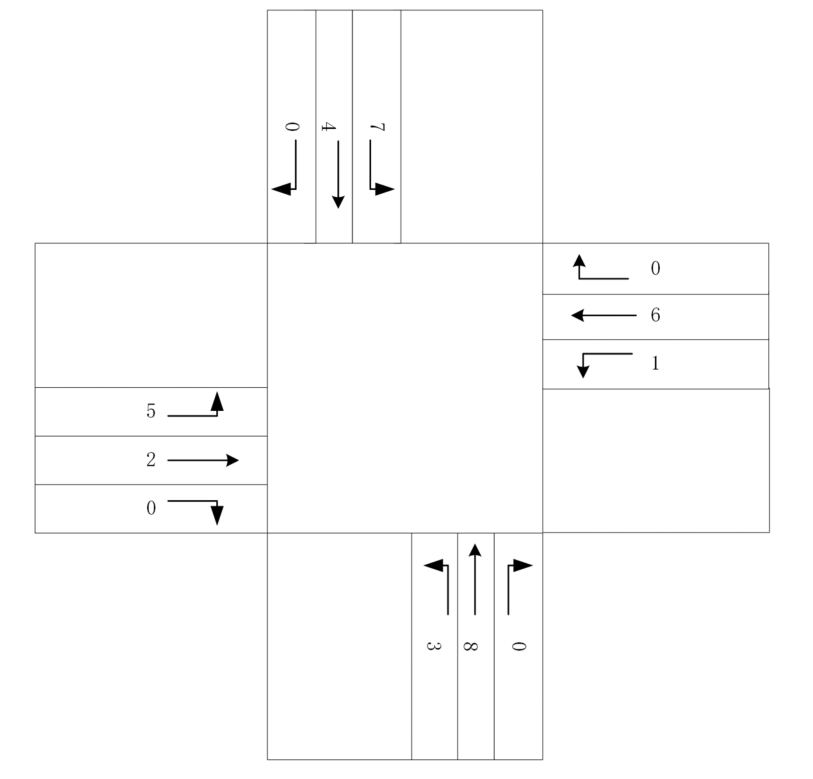
\includegraphics[width=0.75\textwidth]{kuang-lanes}~\caption{Das von Kuang und andere bei einer 3-spurigen Kreuzung dargelegte 8-Phasen Modell~\cite{Zheng2019}}
    \label{fig:kuang-lanes}
\end{figure}

Damit ließe sich der Algorithmus dann noch weiter verfeinern, als dass sie seltene oder fast nie auftretende Szenarien aus der Menge möglicher Zustände entfernen und sich nur die einzelnen Zahlen als Eingabe erhalten muss, nicht die gesamte Struktur der Kreuzung.

Im Folgenden gehen sie auf weitere Arbeiten ein, die eine andere Größenskalierungen als sie vorgenommen haben, bevor sie dann auf die genaue Implementation des Straßenmodells und dem Lernen beziehungsweise Trainieren der künstlichen Intelligenz eingehen.

Ein Problem bei der Phaseneinteilung ist aber, dass sie bei einzelnen Kreuzungen annahmen, dass jede Kreuzung je 3 eingehende Straßen hat, die in die Kreuzung münden.
Auch wenn die Stauzonen meist große Kreuzungen sind, so haben Städte auch Lichtsignalschaltungen verschiedene Kreuzungen mit mehr als nur 3 oder teilweise auch nur 2 Spuren, sodass ein Q-Learning-Algorithmus nicht mit solchen Szenarien umgehen kann und bei anderen Kreuzungen von vorne konzipiert und trainiert werden muss.

Dennoch ist die Einteilung der verschiedenen Lösungsansätze ein wichtiger Aspekt, der auch in dieser Arbeit Relevanz hat, explizit der erste Typ, die feststehende Zeitschaltung.


\textbf{Valentina Kurtc und Martin Treiber:}
\textit{Simulating bicycle traffic by the intelligent-driver model-Reproducing the traffic-wave characteristics observed in a bicycle-following experiment}

Der Forschungsbeitrag von Kurtc und Treiber aus dem Jahr 2020 untersucht die Hypothese, dass sich die Bewegungsdynamik des Fahrzeugverkehrs qualitativ nicht unterscheidet von dem Fahrradverkehr, indem sie die Qualität eines Fahrzeugmodells beziehungsweise Pkw-Modells ebenso für Fahrräder nutzen können.
Dies beweisen sie mit einem ,,Intelligent Driver Model``\cite{Kurtc2020}, einem mikroskopischen Modell für Autos, und vergleichen dessen Qualität der Kalibrierung und Vorhersagefähigkeit dann mit dem ,,Necessary Decelaration Model``\cite{Kurtc2020}, einem mikroskopischen Fahrradmodell.

Im Folgenden gehen Kurtc und andere darauf ein, wie sie eine Vergleichsbasis über die Formel herstellen und das anhand der Beschleunigungsfunktionen aus den Modellen aufbauen, um dann ein Kreisverkehrsszenario mit einem Fahrraddatenset zu simulieren und die berechneten Ergebnisse zu vergleichen.

\begin{figure}[h]
    \centering
    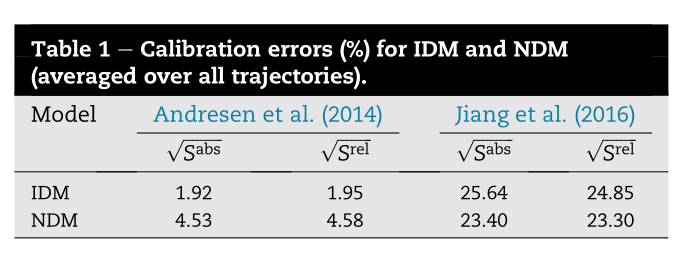
\includegraphics[width=0.75\textwidth]{kurtc2020}~\caption{die von Kurtc und Treiber berechneten, durchschnittlichen Kalbirierungsfehler der beiden Modelle in \%~\cite{Kurtc2020}}
    \label{fig:kurtc2020}
\end{figure}

Das Ergebnis aus der Grafik~\ref{fig:kurtc2020} zeigt, dass die Unterschiede der Modelle beim Nutzen von Fahrraddaten klein sind, als dass sie keinen großen Effekt auf die Simulationen haben.

Aus Kurtc und Treibers Forschungsarbeit lässt sich für diese Simulation also ableiten, dass Agenten, die auf der Straße fahren und Modalitäten wechseln, sowohl mit den Bewegungsmodellen von Fahrrad und Auto simuliert werden können, ohne an Akkuratheit einbüßen zu müssen.


\textbf{Saif Islam Bouderba und Najem Moussa:}
\textit{Reinforcement Learning (Q-LEARNING) traffic light controller within intersection traffic system}

In dem Thesenpapier von Bouderba und Moussa aus dem Jahr 2020 wird eine ähnliche Hypothese wie die von Kuang und andere untersucht.
Sie untersuchen die Effektivität von drei Lösungsansätzen für ihr zelluläres Automatenmodell sind:
Bei dem ersten Experiment simulieren sie einen einfachen, synchronisierten Ablauf der Lichtsignalschaltungen, beim Zweiten einen Ansatz einer ,,Grünen Welle``-Schaltung mit aufeinanderfolgenden Ampeln und beim Dritten eine durch Q-Learning-Algorithmus gesteuerte Kreuzungen~\cite{Bouderba2019}.

Ihr Automatenmodel besteht dabei aus einer Matrix an Kreuzungen, die alle von der Position her mit ihren umliegenden Nachbarn über eine zweispurige Straße verbunden sind:

\[N \times N = 4\]

Jede Kreuzung hat also vier Eingangs- und Ausgangspunkte sowie eine Lichtsignalanlage, die mit je einer Lösungsstrategie pro Experiment gesteuert wird.
Zudem ist die Simulationsumgebung aufgeteilt in Zellen, auf denen sich die Agenten entlangbewegen und zu den Kreuzungen gelangen\cite{Bouderba2019}.

\begin{figure}[h]
    \centering
    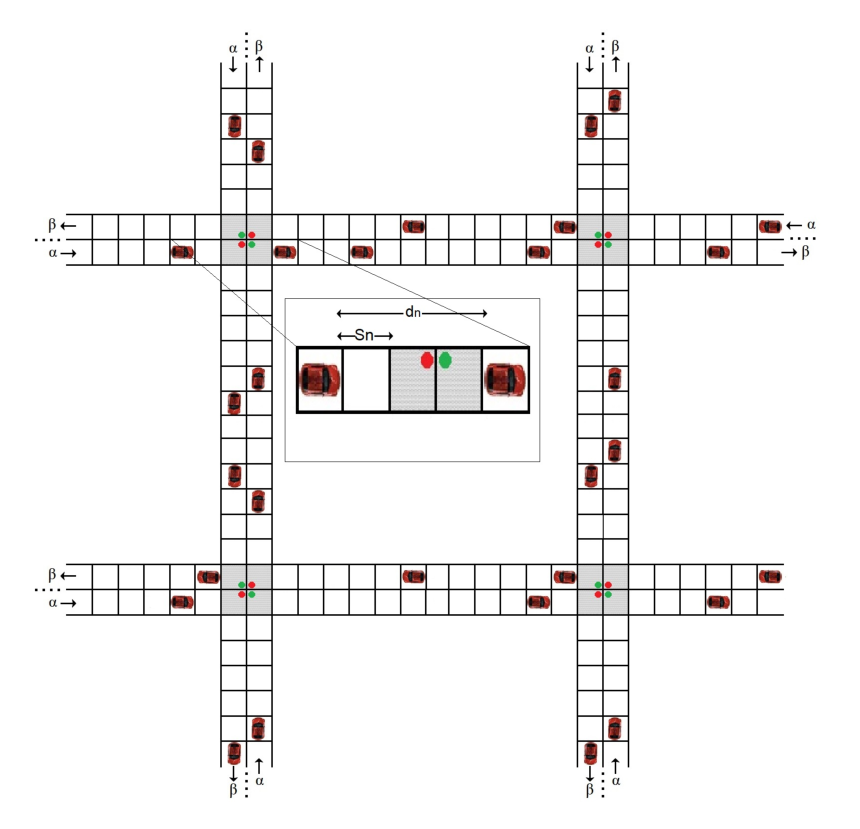
\includegraphics[width=0.75\textwidth]{bouderba-cells-model}~\caption{Eine Momentaufnahme aus dem zellulären Automatenmodell~\cite{Bouderba2019}}
    \label{fig:bouderba-cells-model}
\end{figure}

Mit dem Modell~\ref{fig:bouderba-cells-model} als Simulationsgrundlage erläutern Bouderba und Moussa die Lösungsstrategien.
Die grüne Welle Synchronisation erfolgt über eine Verschiebung der aktuellen, internen Zeituhr von umliegenden Lichtsignalen, während der Q-Learning-Alhorithmus trainiert wird, um eine passende Schaltung selbst zu erlernen.

\begin{figure}[h]
    \centering
    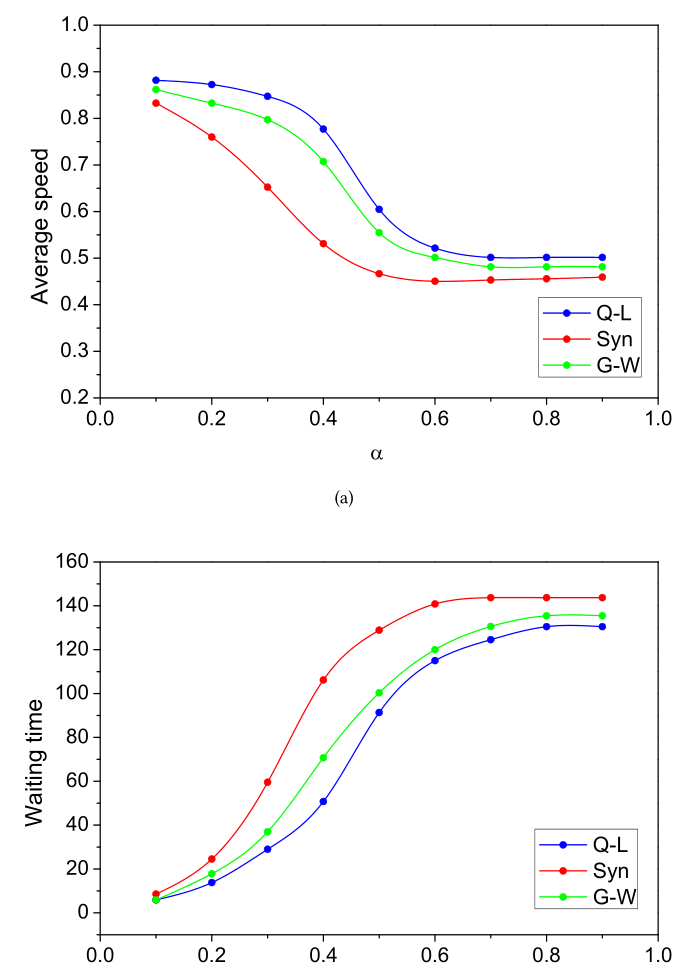
\includegraphics[width=0.5\textwidth]{bouderba-results}~\caption{Die durchschnittliche Geschwindigkeit und Wartezeit nach Durchführunge~\cite{Bouderba2019}}
    \label{fig:bouderba-result-graph}
\end{figure}


Die Resultate in Geschwindigkeit und Wartezeit pro Eingriffsrate aus Grafik~\ref{fig:bouderba-result-graph} zeigen auf, dass der einfache, synchronisierte Ansatz am schlechtesten von allen drei Algorithmen abschneidet.
Die durchschnittliche Wartezeit ist höher als die von dem Q-Learning-Algorithmus und der grünen Welle, genauso wie die durchschnittlichen Geschwindigkeitsmessungen niedriger ausfällt als bei den anderen beiden Ansätzen.

Auch wenn die Grüne-Welle-Schaltung in den Experimenten besser abschnitt, so ist dieser Ansatz nicht der dieser Arbeit.
Der Unterschied besteht darin, dass in Bouderba und Moussas Forschungsarbeit die Ampelphasenlängen auf ihrer Distanz basierend verlängert wurden.
Dies soll in dieser Arbeit aber durch eine insgesamt geltende Phasenschaltung ersetzt werden, da Agenten hier mehr als nur Geschwindigkeit erhöhen und senken können.
Sie können zum Beispiel kleine Veränderungen an Routen unternehmen, sodass sie nicht auf der Straße, sondern auf Fahrradwegen vorbeifahren und Lichtsignalschaltungen ignorieren.
Diese Bewegungsfreiheit der Agenten ist in dem Modell von Bouderba und Moussa nicht gegeben, weshalb die Forschungsarbeit nur als Motivation für die Verbesserungsmöglichkeiten einer grünen Welle angesehen werden kann.


\textbf{Katharina Mulack:}
\textit{Multiagenten Simulation von Fahrradfahrern im Kontext urbaner Verkehrsdynamik}

Die Masterarbeit von Katharina Mulack aus dem Jahr 2020 basiert ebenso auf dem MARS-Framework und ergänzt die bis zu dem Zeitpunkt der Arbeit in dem Framework fehlenden Fahrradfahrer.
Dabei fokussiert sich die Arbeit auf die detailreiche Rekonstruierung von Fahrradfahrern mit einem eigenen Bewegungsmodell, Statistiken über Eigenschaften von Fahrrädern und deren Interaktion mit der Umgebung\cite{Mulack2020}.
Bei den Verkehrsflussmodellen, einem Kernaspekt der Forschungsarbeit, wird insbesondere auf vier unterschiedliche Modellierungskonzepte eingegangen, die sich in der Feinheit der Simulationsmodelle unterscheiden:

Makroskopische Flussmodelle, die bei Simulationen sich mit dem allgemeinen Verlauf beschäftigen und die Details wie die Simulation einzelner Fahrzeuge nicht simulieren, um das Gesamtverhalten und ihr Effekt der Bewegung zu beobachten\cite{Mulack2020}.

Mikroskopische Modelle wiederum dienen der detaillierteren Simulation und beziehen individuelle Verhaltensweisen von Agenten mit der Umwelt oder anderen Agenten ein\cite{Mulack2020}.

Submikroskopische Modelle wiederum sind noch spezifischer und simulieren sogar Beziehungen zwischen Agenten und Entitäten, um den Detailgrad der echten Welt zu imitieren\cite{Mulack2020}.

Zuletzt wird noch das Mesoskopische Modell genannt, welches eine Mischung aus Makro- und Mikroskopmodell ist.
Bei diesem werden sowohl über große Distanzen und Gesamtverhalten angeschaut werden, dennoch aber die einzelnen Agenten oder Entitäten diese große Veranschaulichung ausmachen\cite{Mulack2020}.

Im Folgenden untersucht Mulacks Masterarbeit die Verkehrsflussmodelle und Statistiken über Fahrräder und implementiert sie zusammen mit neuen Umwelteinflüssen, den Lichtsignalanlagen.

Mulacks Forschungsarbeit selbst befasst sich mit einem hohen Detailgrad und zwischenagentlichen Beziehung bei den Fahrradfahrern, während sich diese Arbeit hier eher mit einem gemischten, mesoskopischen Simulationsmodell beschäftigt.
Zwar wird in dieser Arbeit ebenfalls auf einzelne Agenten benutzt, die mit ihrer Umwelt und den Entscheidungen andere Agenten beeinflussen, aber ist die generelle Stau- und Warteschlangenbildung wichtiger für die Ergebnisse.

Auch beschäftigt sich die Arbeit mehr mit dem Verhalten der Fahrradfahrer selbst innerhalb des MARS-Frameworks, nicht mit der Entwicklung einer optimalen Lichtsignalschaltung.
Dies macht diese Masterarbeit zu einer geeigneten Quelle für detailreiche Verhaltensweisen von Fahrrädern, weniger aber zu einem vergleichbaren Ansatz für diese Arbeit.


\textbf{Thomas Clemen, Nima Ahmady-Moghaddam, Ulfia A. Lenfers, Florian Ocker, Daniel Osterholz und Jonathan Ströbele:}
\textit{Multi-Agent Systems and Digital Twins for Smarter Cities}

In der Forschungsarbeit aus dem Jahr 2021 beschäftigen sich Clemen und andere mit dem ,,Internet of Things``, fortan als IoT abgekürzt, welches eine Großzahl an (Echtzeit-) Daten über die Stadt Hamburg via Sensoren anbietet, und entwickeln dazu ein digitales Zwillingsmodell der Stadt selbst, zur Überführung der Daten in das MARS-Framework.
Im Zentrum dabei steht nicht nur die Nutzungsermöglichung der IoT-Daten, sondern ebenfalls die Frage: Wie baut werden ort- und zeitlich gebundene Daten in ein Echtzeitmodell integriert, in der sich die Simulationen und Experimente anschaulich darstellen und kontrollieren lassen sollen~\cite{Clemen2021}?

Ihr Lösungsweg: Das Herunterbrechen der Akteure in der echten Welt auf Agenten und Entitäten, die damit als eine digitale Zwillingsinstanz~\cite{Clemen2021} fungieren und das Verhalten der Akteure oder Simulationsflächen imitieren.
Dabei wird zudem noch ein Fokus darauf gelegt, zwischen passiven, aktiven und interagierbaren Zwillingsinstanzen zu unterscheiden, da der Verhaltens- und Implementationsaufwand durch die Entscheid- und Bewegungsfreiheit steigt.
Entsprechend entscheiden sie sich, in ihrer Forschung vorerst die Echtzeitdaten nur bei passiven Zwillingsinstanzen zu implementieren.
Als Grundlage dafür wird das SmartOpenHamburg-Projekt genommen, was bereits die physische Repräsentation der Stadt sowie eine Reihe der städtischen Modalitäten implementiert hat, und erweitern dieses um den Zugang zu den IoT-Daten~\cite{Clemen2021}.

Dadurch, dass in der Forschungsarbeit von Clemen und andere nur die passiven, digitalen Zwillinge mit Daten angereichert werden, fehlt für die Arbeit hier die Echtzeitdaten von Lichtsignalschaltungen sowie einem Echtzeitverkehrssensor.
Da in der Arbeit von diesem Papier hier sich auf den Verkehrsfluss und explizit auf die Simulation einzelner Agenten fokussiert wird, müssen diese aktiven Agenten sein, die Entscheidungen über Modalitäten, Wege und Interaktion mit Entitäten unternehmen.
Damit würden sie unter die interagierbaren, digitalen Zwillinge fallen, die mit Eingabedaten bestückt werden müssten und sind entsprechend mit einem großen Mehraufwand beim Implementieren verbunden.

Entsprechend ist die Forschung der Arbeit von Clemen und andere zwar eine gute Grundlage für zukünftige Ausblicke dieser Arbeit, sollten Echtzeitdaten bereitgestellt werden für aktuellen Verkehr an Lichtsignalanlagen oder generell auf Straßen.
Jedoch ist der Nutzen für diese Arbeit beschränkt auf das SmartOpenHamburg-Projekt, dass die Grundlagen zur agentenbasierten Simulation bereits bereitstellt.


\textbf{Daniel Glake, Fabian Panse, Norbert Ritter, Thomas Clemen und Ulfia Lenfers:}
\textit{Data Management in Multi-Agent Simulation Systems}

Daniel Glake und andere beschäftigten sich im Jahr 2021 in ihrem Forschungsbeitrag mit den Problemen des Einbauens von unterschiedlichen Daten in einem sehr groß skalierten Simulationsszenario und präsentieren dabei Lösungen für die Herausforderungen mithilfe des MARS-Frameworks.
Dabei fokussieren sie sich auf fünf großen Eingabedatenkategorien, die in der MARs-Simulationsumgebung eingebaut werden und mit großskalierten Projekten zu Herausforderungen kommen können:
\begin{itemize}
    \item Eingabedaten für Simulationen, die zum Beispiel bei einem Ortstransfer zu Kompabilitätskomplikationen führen, wie etwa mit geografischen Karten, den lokalen Infrastrukturnetzwerken oder weitere, nicht-ortsgebundene Daten wie zeitliche Busfahrpläne~\cite{Glake2021}.
    \item Ausgabedaten von großen Simulationen, die beim Simulieren eine Großzahlan Agenten und Entitäten nutzen, blockieren beziehungsweise verzögern beim Exportieren von Zwischenständen die aktive Simulation deutlich und schränken damit die Fähigkeit diese in Echtzeit zu analysieren ein~\cite{Glake2021}.
    \item Eingabedaten über Streams werden beim Vorhersagen von Simulationszuständen, wie etwa den Agentattributen oder Umweltinformationen, immer ungenauer je weiter in die Zukunft berechnet wird.~Dafür bieten Schnittstellen und angebundenen Systeme Möglichkeiten zum vermindern dieser Ungenauigkeit.~Das Korrigieren benötigen aber dennoch bei einer großen Anzahl von Agenten einem Moment zum Überreichen, was zeitlich ebenfalls zu Verzögerungen führen und auch die Echtzeitanalysefähigkeit erschwert~\cite{Glake2021}.
    \item Bei Schnittstellen für räumlich-zeitliche Abfragen wird stets der jeweilige Raum benötigt und zum Beispiel in MARS als Polygon angegeben.~Operationen wie ,,beinhält``, ,,überlappt`` oder ,,ist adjazent von`` sind dabei häufig genutzt, was bei einer Vielzahl von Agenten, die dies gleichzeitig durchführen und sich dabei bewegen, zu zeitlichen sowie geographischen Unterschieden führt~\cite{Glake2021}.
    \item Beim Planen dieser räumlich-zeitlichen Abfragen, wie das System die echte Welt auf die Modellrepräsentation abzubilden hat, darf die Migrationszeit nicht die Datenverarbeitungszeit überschreiten, damit es nicht zu Inkonsistenzen in der Simulation führt.~Strategien, die das verhindern, sind aber nur Annäherungen, da die Optimierung der Migrationszeit einem NP-Problem entspricht und somit nicht mit einer konstanten Anzahl an Operationen berechnet werden kann~\cite{Glake2021}.
\end{itemize}

Danach gehen Glake und andere genauer darauf ein, wie sie diese Problematiken im MARS-Framework mit Lösungsansätzen vermindert oder gelöst bekommen haben.
Für diese Arbeit hat die Forschungsarbeit von Glake und andere aber keinen relevanten Bezug:
Das System hier ist kein Echtzeitsystem auf einem großskalierten Bereich.
Der Simulationsraum beschränkt sich auf die Binnen- und Außenaslter und zur Ergebnissermittlung genügt es bereits, wenn die Simulation nebenbei berechnet wird.
Eine Verzögerung aufgrund von groß skalierten Bereichen oder zu vielen Agenten affektiert nicht die Korrektheit des Systems und ist sich also nicht von den kategorisierten Problemen affektiert.

Dennoch wären für zukünftige Arbeiten das Papier von Glake und andere ein guter Ansatz, um Echtzeitdaten mit der gesamten Stadt Hamburg zu verbinden und damit den gesamten Raum zu simulieren, nicht nur wie hier um die Binnen- und Außenalster.


\textbf{Ulfia A. Lenfers, Nima Ahmady-Moghaddam, Daniel Glake, Florian Ocker, Daniel Osterholz, Jonathan Ströbele und Thomas Clemen:}
\textit{Improving Model Predictions—Integration of Real-Time Sensor Data into a Running Simulation of an Agent-Based Model}

In einem weiteren Forschungsartikel über das MARS-Framework im SmartOpenHamburg-Projekt des Jahres 2021 beschäftigen sich Ulfia A. Lenfers und andere mit der Verbesserung der Einbindungsimplementation von Echtzeitdaten und zeigen das Potenzial anhand von Fahrradverleihstationen, wie mit der Modellierung und Daten genauere Vorhersagungen zu Fahrradverleihs getroffen werden können.

\begin{figure}[h]
    \centering
    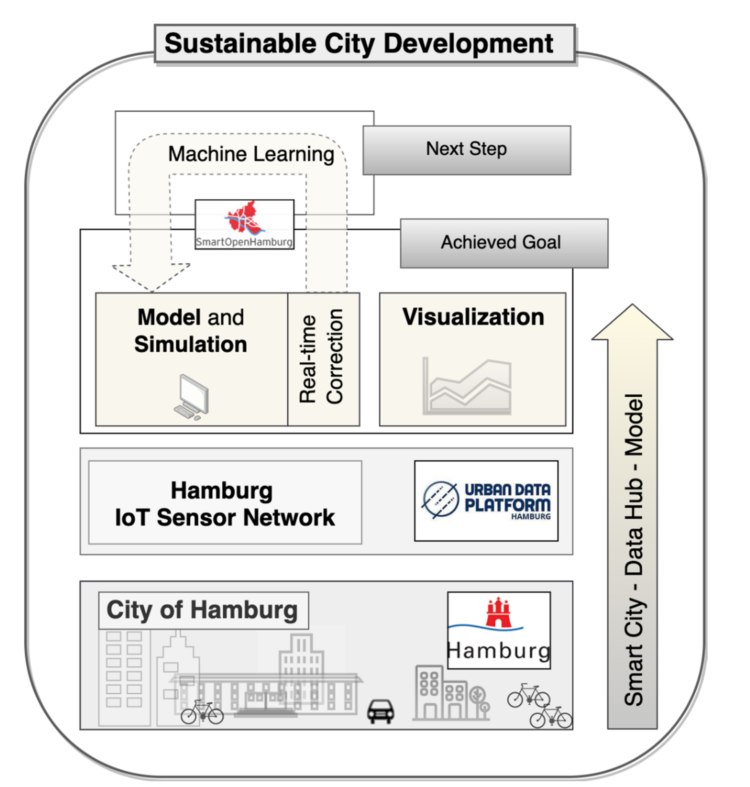
\includegraphics[width=0.75\textwidth]{lenfers-workflow}~\caption{Beispielworkflow, wie Daten aus den Sesnsoren und von der Stadt Hamburg in ein abstraktes Simulationsmodell eingebaut werden~\cite{Lenfers-MP-2021}}
    \label{fig:lenfers-workflow-sensors}
\end{figure}

Wie aus dem Workflow von~\ref{fig:lenfers-workflow-sensors} zu entnehmen ist, fokussiert sich der Kern der Arbeit aus dem Zusammenspiel von Datenfluss des Smart-City-Data-Hub und die Dateneinbindung von Fahrradverleihstationen in die SmartOpenHamburg-Komponente.
Echtzeitdaten werden bei ihrer Implementation von der ,,Smart City`` über ein zeitlichen Vektor-Layer in die Simulation konstant eingelesen und anhand ihrer Lebenszeit entsprechend simuliert\cite{Lenfers-MP-2021}.
Die Daten selbst werden dabei über eine URI von den externen Endpunkten abgefragt und mit zusätzlichen Argumenten auf die relevanten Daten reduziert~.
Mit diesem Datenstrom werden die derzeitigen Zustände der Fahrradverleihstationen abgefragt und in die Simulation eingebaut, wie viele Fahrräder derzeit aktuell aktiv genutzt werden und wie viele Agenten in der Simulation agieren\cite{Lenfers-MP-2021}.

Der Forschungsbeitrag von Lenfers und andere ist aber, wie bei der vorherigen, für diese Arbeit nur begrenzt relevant: Die statische Implementation von Fahrradverleihstationen ist relevant, da Verkehrsteilenhmer an den Stationen sich ein Fahrrad leihen können, doch ist dabei kein Echtzeitstrom vonnöten und passiert passiv nebenbei.

Dennoch bietet die Arbeit Anknüpfmöglichkeit, sollten relevanten Echtzeitdaten von der Stadt Hamburg zum Verkehr oder zu Lichtsignalanlagen über die nächste Zeit aufkommen und damit den Kern einer anderen Arbeit darstellen.


\textbf{Daniel Glake, Fabian Panse, Norbert Ritter, Thomas Clemen und Ulfia Lenfers:}
\textit{Incorporating Multi-Modal Travel Planning into an Agent-Based Model: A Case Study at the Train Station Kellinghusenstraße in Hamburg}

Der Forschungsartikel von Lenfers und andere aus dem Jahr 2021 erweitert ebenfalls das MARS-Framework und das SmartOpenHamburg-Projekt um nachhaltige Modalitäten wie die mietbaren Äquivalente zu Pkws und Fahrrädern oder das Zu-Fuß-Gehen.
Dabei untersuchen sie, wie effizient das Wechseln der Modalitäten in einem Beispielszenario ist und ob die Optimierungsstrategien hinsichtlich der Klimaneutralität, aus finanziellen Gründen oder persönlichen Präferenzen korrekt annähern~\cite{Lenfers-MMT-2021}.

Das Beispielszenario, welches sie zur Demonstrierung der implementierten Modalitäten verwenden, umfasst dabei die Bahnhofsstation Kelinghusenstraße in Hamburg, von der aus die Agenten mit den Modalitäten in einem Kreis-Bereich zu ihrem Ziel gelangen können.

\begin{figure}[h]
    \centering
    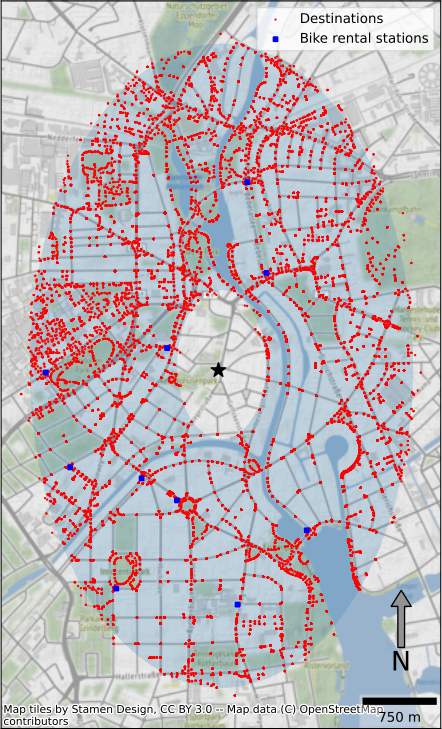
\includegraphics[width=0.75\textwidth]{lenfers-kelinghusen}~\caption{Karte der Fahrradverleihstationen, mit dem Simulationsbereich der Agenten hellblau hinterlegt, den Interessenspunkten rot markiert und Fahrradverleihstation als blaue Markierungen~\cite{Lenfers-MMT-2021}}
    \label{fig:lenfers-kelinghusen-area}
\end{figure}

Auf dem Weg zu ihrem Endziel innerhalb des simulierbaren Bereichs aus~\ref{fig:lenfers-kelinghusen-area} kommen manche Agenten durch angestrebtes Nutzen der Modalitäten erst zur nächsten Fahrrad- oder Pkwverleihstation, bevor sie ihre Reise zum Interessenspunkt fortsetzen können.
Dieses angestrebte Nutzen wird in den Eingabedaten durch zum Beispiel die Variablen ,,hasCar`` und ,,usesBikeAndRide`` versinnbildlicht, wie hoch die Wahrscheinlichkeit zum Nutzen oder Besitzen einer eigenen oder gemieteten Modalität ist~\cite{Lenfers-MMT-2021}.

Auf den implementierten Modalitäten und Verleihstationen aus der Forschungsarbeit von Lenfers und andere knüpft diese Arbeit hier an und untersucht nun mithilfe der Auswahl an Modalitäten eine mögliche Lichtsignalschaltung.
Damit bietet diese Arbeit eine sehr gute Grundlage, auf der nun aufgesetzt und das hier in dieser Arbeit beschriebenen Szenario aufgesetzt wird.


    % The third chapter about the code's conzept
% @author Kalvin Döge
%


\chapter{Konzept}\label{ch:konzept}

Im Folgenden wird das Model der Simulation konzeptioniert und ausgeführt, mit den vorherigen Begriffserklärungen als Grundlage.
Dabei wird auf den Simulationsort im Modell, den Aufbau und Voreinstellungen der Agenten und Lichtsignalschaltungen, die Projektarchitektur und zuletzt noch auf den Umfang der Arbeit eingegangen.

% The section about the simulation's type
% @author Kalvin Döge
%


\section{Simulationstyp}\label{sec:simulationtype}

Für diese Arbeit empfiehlt sich eine agentenbasierte Simulation, da im Vornherein die zu fahrende Route eines Agenten zwar bekannt ist, die Einflüsse von zum Beispiel Pkws aber direkt im Übergang von einer Lichtsignalschaltung zur anderen den Akteur beeinflussen und so nicht vorhergesehen werden können.
Damit also keine Annahmen über dynamische, umwelt- oder agentenbedingte Einflüsse im Quellcode festgelegt werden, ist entsprechend eine agentenbasierte Echtzeitsimulation angemessener für diese Simulation.

% The section about the place of the simulation itself
% @author Kalvin Döge
%


\section{Simulationsort}\label{sec:simulationplace}

Für die Arbeit wurde die Binnen- und Außenalster als Simulationsumgebung ausgewählt.

\begin{figure}[h]
    \centering
    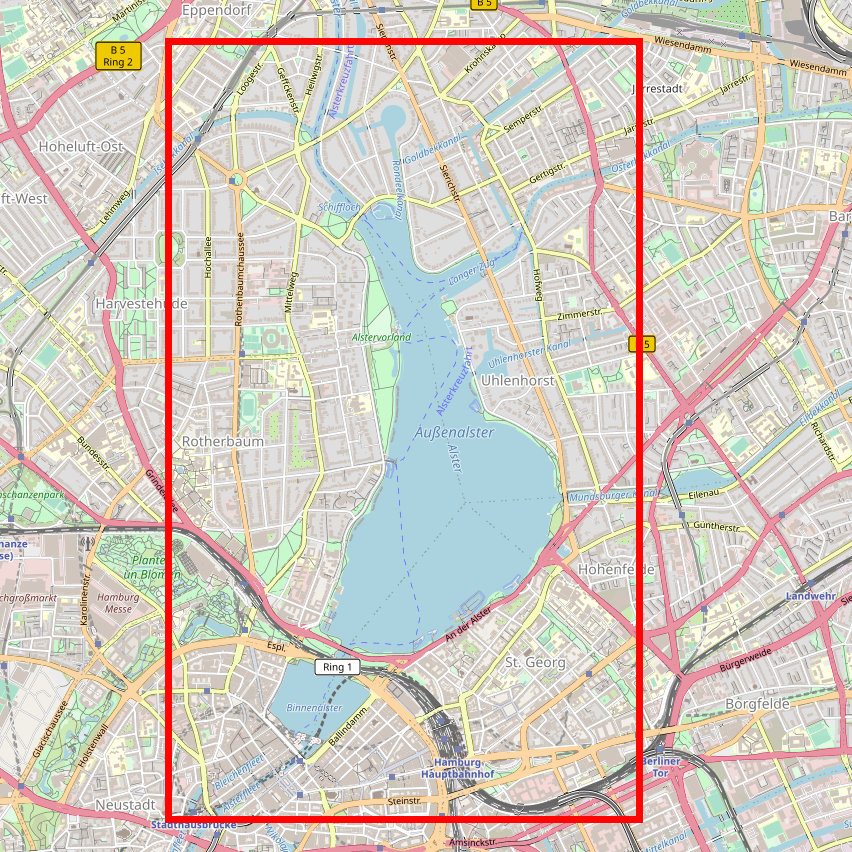
\includegraphics[width=0.75\textwidth]{sim-area}
    \caption{Simulationsumgebung}
    \label{fig:sim-area}
\end{figure}

Wie im Ausschnitt~\ref{fig:sim-area} zu erkennen ist, ist aufgrund der zentralen Lage innerhalb der Stadt, vieler anliegenden Kreuzungen und generell dichter Besiedelung um die Alster herum eine hohe Dichte an Agenten für die Simulation gegeben, die eine ,,Grüne Welle`` für Fahrradfahrer erschweren können.
Dies gibt der Simulation auf der einen Seite eine Herausforderung, mit schwereren Vorgaben überhaupt eine Lichtsignalschaltung für die ,,Grüne Welle`` zu finden, während auf der anderen Seite dafür aber diese Simulation wie eine ,,Obergrenze`` angesehen werden kann für die Agenten- und Lichtsignalanzahlen.

% The section about the agents of the simulation itself
% @author Kalvin Döge
%


\section{Agenten}\label{sec:agents}

Im Folgenden werden die Konzepte der Agenten näher erläutert, wobei besonders auf die Grundlagen der Agenten, ihre Modalitäten, die Interaktion mit anderen Agenten und Entitäten, die Anzahl an aktiven Agenten und auf die gefahrene Routen eingegangen wird.

% The section about the agents' modalities of the simulation itself
% @author Kalvin Döge
%

\subsection{Voraussetzungen}\label{subsec:prerequisities}

Es gibt zwei Arten von Agenten, die in der Simulation agieren: Den Nebenagenten, fortan ,,\code{HumanTraveler}`` genannt, und dem Hauptagenten, fortan ,,\code{BicycleLeader}`` genannt.

Der \code{BicycleLeader} ist der Fokus dieser Arbeit.
Dieser wird immer mit einem eigenen Fahrrad oder einem mietbaren Fahrrad ausgestattet, mit dem er vorgegebene Punkte auf einer Route um die Alster abfahren soll.
Sein Ziel ist es, eine Runde um die Alster zu fahren, ohne dabei auf 0 km/h bremsen zu müssen.
Langsames Fahren ist hier nicht mit einbezogen als Fehlschlagbedingung, da eine Schwelle für ,,zu langsames`` Fahren, sodass der \code{BicycleLeader} sein Gleichgewicht nicht mehr halten könne, von einer Reihe von Faktoren abhängt, die außerhalb des Rahmens dieser Arbeit wären: das Alter des BicycleLeaders, die Erfahrung mit dem Fahrrad, das angestrebte Fahrverhalten, Höhenprofile der Umgebung, Wetterbedingungen und noch einige Aspekte mehr.

\code{HumanTraveler} sind dabei die Einwohner, die mit Lichtsignalschaltungen interagieren und auf den Straßen dem \code{BicycleLeader} in die Quere kommen.
Das Ziel der \code{HumanTraveler} ist es lediglich, ein zufällig zugewiesenes Ziel um die Alster herum zu erreichen, bevor sie aus der Simulation entfernt werden.

% The section about the agents' modalities of the simulation itself
% @author Kalvin Döge
%

\subsection{Modalitäten}\label{subsec:modalitaten}

Die \code{HumanTraveler} haben drei Arten der Transportation zur Verfügung: zu Fuß, Pkws und Fahrräder.
In dem MARS-Framework ist es Agenten ebenso gestattet, bei Autos und Fahrrädern diese zu Mieten und damit sogenannte ,,RentalCars'' oder ,,RentalBikes'' zu nutzen, jedoch hat es für diese Arbeit keinen großen Einfluss, ob sie ihr eigenes Transportmittel nehmen oder einen Umweg zu den mietbaren Äquivalenten einschlagen, da die Agenten in der Simulation nur als ,,Störfaktor`` über Ampeln und auf Straßen mit dem Hauptagenten interagieren.

Für jede Modalität gibt es eine vorgesehene Straße zum Befahren: Pkws fahren auf Straßen, Fahrräder fahren auf Fahrradlinien und teilweise auch auf Straßen.
Fußgänger können sich nur auf Fußgängerwegen bewegen, dafür können sie in andere Modalitäten wechseln.
Jeder \code{HumanTraveler} als auch der \code{BicycleLeader} beginnt die Simulation als Fußgänger, bevor sie auf eine Modalität aufsteigen.

% The section about the agents' modalities of the simulation itself
% @author Kalvin Döge
%

\subsection{Interaktionen mit Agenten und Entitäten}\label{subsec:interactions}

Interaktionen zwischen Agenten sind in dieser Simulation beschränkt auf zwei Arten: dem Verlangsamen und Blockieren auf Straßen als auch dem Aufhalten von anderen Agenten an Lichtsignalschaltungen.
\code{HumanTraveler} und \code{BicycleLeader} können über ihre Pkws und Fahrräder an Ampeln einen Platz einnehmen und damit die Warteschlangen verlängern.
Je länger sie wird, desto mehr Zeit benötigt die Simulation, um die Warteschlange bei einem grünen Signal zu leeren.

Auf den Straßen und Fahrradwegen selbst haben die jeweiligen Modalitäten nur dann miteinander Interaktionen, wenn sie sich zu Nahe kommen.
Damit es nicht zu Kollisionen kommt, wird überprüft, wie nahe sich zwei Agenten sind, um dann zu verlangsamen oder weiterzufahren.
Eine detailliertere Abhandlung dazu wird im Kapitel ,,Implementierung`` angegangen.

% The section about the agents' amount of the simulation itself
% @author Kalvin Döge
%

% graphics

\subsection{Anzahl aktiver Agenten}\label{subsec:activeagents}

Zur Bestimmung von der Anzahl an aktiven Agenten, wurde eine angenäherte Rechnung für die Population um die Alster genommen, da direkte Statistiken zur täglichen Anzahl an Verkehrsteilnehmern in Hamburg beziehungsweise in verschiedenen Stadtvierteln fehlen.
Um eine Annäherung an die Verkehrszahlen zu bekommen, wird zuerst die Verteilung über Haupt-, Neben- und Schwachverkehrszeiten untersucht.

Ein Arbeitstag, Montag bis Freitag, hat zwei große Hauptverkehrszeiten: morgens von 6 bis 9 Uhr und nachmittags von 15 bis 19 Uhr~\cite{FHH2015}.
In diesen beiden Zeiten werden die meisten Verkehrsteilnehmer auf den Straßen unterwegs sein und damit am ehesten Staus verursachen.

Die Nebenverkehrszeit tritt von 9 bis 15 Uhr~\cite{FHH2015} auf, die den Übergang zwischen den beiden Hauptverkehrszeiten darstellt.
Innerhalb dieser Zeit ist die Dichte an Verkehrsteilnehmern geringer als in der Hauptverkehrszeit, aber immer noch höher als in Schwachverkehrszeiten.

Die Schwachverkehrszeit ist von 20 Uhr bis 5 Uhr am nächsten Tag~\cite{FHH2015}, in der der Verkehr am geringsten ist, die Straßen leer und der Stau am seltensten auftritt.


Um den Verlauf über einen Tag nun mit zwei Hochpunkten und drei Tiefpunkten darzustellen, während dabei der zweite Tiefpunkt höher als der erste und dritte ist, könnte man eine negierte Funktion 4.\ Grades benutzen.

\begin{figure}[h]
    \centering
    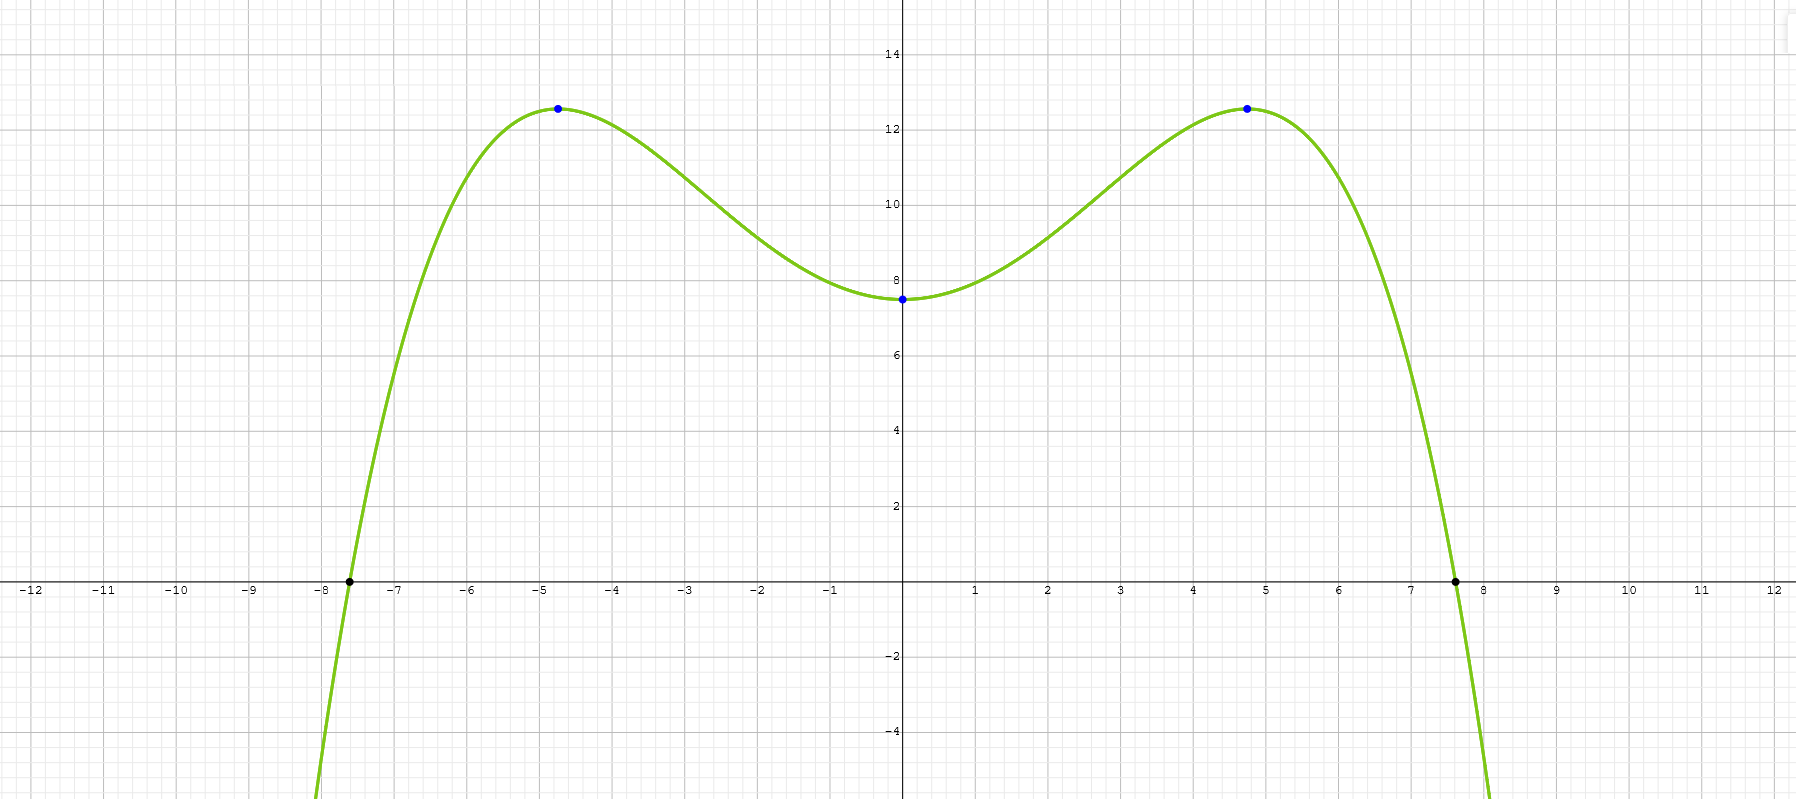
\includegraphics[width=1.00\textwidth]{poly-4-degree}
    \caption{Polynomialfunktion des 4. Grades zur Annäherung}
    \label{fig:poly-4-degree}
\end{figure}

Die Funktion aus der Grafik~\ref{fig:poly-4-degree} lautet: \[f(x)=-0.01x^4+0.45x^2+7.5\]

Die Grafik~\ref{fig:poly-4-degree} muss so interpretiert werden, als hätte die x-Achse eine Verschiebung von 12 Einheiten nach rechts noch erhalten, damit die Werte sich passend der Tagesstunden verteilen.
Entsprechend ist 0 Uhr hier bei x = -12, 12 Uhr ist bei x = 0 und 24 Uhr ist bei x = 12.

Zum Annähern selbst ist die Funktion aber nur ansatzweise nützlich, da wenn x die Stundenanzahl und f(x) der Prozentsatz aller aktiven Agenten darstellt, die Schwachverkehrszeiten bei einer Funktion 4.\ Grades auf der x-Achse in das Negative gehen würden.
Damit wäre aber, wenn f(x) Nullstellen bei \[x = -12, x = 12\] hätte, keine relativ gleiche Verteilung über die 9 Stunden, also wäre von 20 bis 5 Uhr keine relativ flache Schwachverkehrszeit.
Der zweite Ansatz wäre, bei einem anderen x-Wert die Nullstelle schneiden zu lassen, wie es in der Grafik~\ref{fig:poly-4-degree} zu sehen ist, also zum Beispiel an den Stellen \[x = -7.6, x = 7.6\]
x = -7.6 wäre um circa 4 Uhr und x = 7.6 wäre um circa 20 Uhr.
Bei diesem Ansatz werden dann aber negative Funktionswerten außerhalb der x-Werte auftreten und damit ,,negativen Verkehr`` verursachen.
Das kann logischerweise nicht in der realen Welt auftreten, also müssen die Werte auf 0 oder einen anderen Wert gesetzt werden.
Sollte der Wert auf 0 gesetzt werden, wäre das noch immer keine korrekte Darstellung für das Modell, da in der Schwachverkehrszeit noch immer Verkehr vorliegt.
Um einen besseren Funktionsverlauf zu gewährleisten, muss die Funktion interpoliert werden, um flachere Übergänge in die Schwachverkehrszeit zu bewerkstelligen.
Um den Verlauf beziehungsweise die Interpolation zu konstruieren, werden kubische Polynome genutzt, die an bekannten Punkten eine Ober- beziehungsweise Untergrenze bilden und damit übergehen in die nächste, kubische Funktion.
Mithilfe Timo Denks Implementation der kubischen Spline-Interpolation~\cite{Denk2018} lässt sich mithilfe der Datenpunkte aus der Vorabinformation von der Stadt Hamburg annähern.


$f(x) = \begin{cases}
            8.8699 \cdot 10^{-2}\cdot x^3 -1.4163 \cdot 10^{-59}\cdot x^2 + 2.0171 \cdot 10^{-1}\cdot x + 0.0000, & \text{if } x \in [0,3], \\-2.0275 \cdot 10^{-1}\cdot x^3 + 2.6231\cdot x^2 -7.6675\cdot x + 7.8692, & \text{if } x \in (3,6], \\9.4824 \cdot 10^{-2}\cdot x^3 -2.7333\cdot x^2 + 2.4471 \cdot 10^{1}\cdot x -5.6408 \cdot 10^{1}, & \text{if } x \in (6,12], \\-8.5660 \cdot 10^{-2}\cdot x^3 + 3.7641\cdot x^2 -5.3498 \cdot 10^{1}\cdot x + 2.5547 \cdot 10^{2}, & \text{if } x \in (12,18], \\1.2958 \cdot 10^{-1}\cdot x^3 -7.8589\cdot x^2 + 1.5572 \cdot 10^{2}\cdot x -9.9981 \cdot 10^{2}, & \text{if } x \in (18,22], \\-1.1557 \cdot 10^{-1}\cdot x^3 + 8.3212\cdot x^2 -2.0025 \cdot 10^{2}\cdot x + 1.6106 \cdot 10^{3}, & \text{if } x \in (22,24].
            \label{fig:interpolation}
\end{cases}$

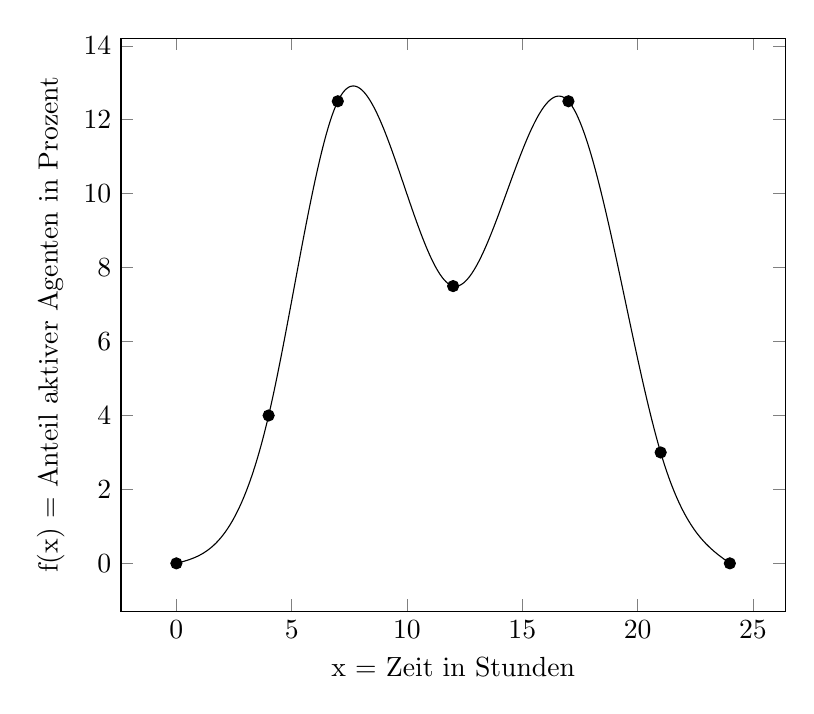
\begin{tikzpicture}
    \pgfplotsset{
        scale only axis,
    }

    \begin{axis}
        [
        xlabel={x = Zeit in Stunden},
        ylabel={f(x) = Anteil aktiver Agenten in Prozent},
        samples=100,
        ]
        \addplot [only marks] table {
            0 0
            4 4
            7 12.5
            12 7.5
            17 12.5
            21 3
            24 0
        };


        \addplot[][domain=0:4]{+0.05212125853316996*x^3+3.4e-60*x^2+0.1660598634692806*x^1+0*x^0};
        \addplot[][domain=4:7]{+-0.19010136076913603*x^3+2.9066714316276716*x^2+-11.460625863041406*x^1+15.502247635347583*x^0};
        \addplot[][domain=7:12]{+0.12557646303751677*x^3+-3.722562868312037*x^2+34.94401423653655*x^1+-92.77524593033432*x^0};
        \addplot[][domain=12:17]{+-0.11369945737791003*x^3+4.891370266643328*x^2+-68.42318338292783*x^1+320.6935445475232*x^0};
        \addplot[][domain=17:21]{+0.12176450638893752*x^3+-7.117291885465897*x^2+135.724073202929*x^1+-836.1409094389987*x^0};
        \addplot[][domain=21:24]{+-0.061541335226351856*x^3+4.430976136297334*x^2+-106.78955525409884*x^1+861.454489760196*x^0};
    \end{axis}
    \label{fig:interpolation-graph}
\end{tikzpicture}


Nun muss nur noch die Einwohnerdichte pro km\textsuperscript{2} angenähert werden, damit man eine grobe Gesamtanzahl an Agenten ableiten kann.
Das Statistikamt Nord, das für Schleswig-Holstein und Stadtteile Hamburgs Statistiken sammelt, hat in ihrem Bericht aus dem Jahr 2021 die Einwohnerdichte aller Stadtteile Hamburgs aufgelistet~\cite{SAHHSH2022}.
Der Simulationsort dieser Arbeit umfasst die folgenden Stadtteile: Neustadt, St. Georg, Hohenfelde, Uhlenhorst, Winterhude, Eppendorf, Harvestehude und Rotherbaum.
Für diese Stadtteile wird die Einwohnerdichte pro km\textsuperscript{2} ausgelesen:

\begin{center}
    \begin{tabular}{||c c c c||}
        \hline
        Stadtteil    & Einw.\ je km\textsuperscript{2} \\ [0.5ex]
        \hline\hline
        Neustadt     & 5575                            \\
        \hline
        St. Georg    & 6291                            \\
        \hline
        Hohenfelde   & 8578                            \\
        \hline
        Uhlenhorst   & 8516                            \\
        \hline
        Winterhude   & 7499                            \\
        \hline
        Eppendorf    & 9193                            \\
        \hline
        Harvestehude & 8636                            \\
        \hline
        Harvestehude & 6253                            \\
        \hline\hline
        Gesamt       & 60.541         \\[1ex]
        \hline
    \end{tabular}
\end{center}

Es werden absichtlich aus dieser Statistik manche Agentengruppen nicht entfernt oder hinzugefügt, da keine genauen Statistiken dazu von der Stadt Hamburg gegeben oder bei der Recherche aufgefunden werden konnten zum Verwenden in dieser Arbeit.
Jene Gruppen umfassen, sind aber nicht beschränkt auf: Kinder, Eltern, die Zuhause auf Kindern aufpassen, Home-Office-Workers, Alte oder kranke Leute, Arbeitslose und noch mehr.
Diese müssten theoretisch gesehen aus den Statistiken entfernt werden, während folgende Menschengruppen zu der Statistik hinzugezählt werden müssten: Pendler aus anderen Städten, Pendler aus anderen Stadtvierteln, Privatpersonen mit mehr als einem Fahrtziel, Berufsfahrer wie zum Beispiel Taxis oder Lieferanten, Touristen und so weiter.
Der Einfachheit halber wurde also die durchschnittliche Einwohnerzahl der betroffenen Stadtviertel genommen, anstatt alle Umweltfaktoren aus der echten Welt einzubeziehen.

Mit der Gesamtmenge an Einwohnern pro km\textsuperscript{2} lässt sich der Durchschnitt aller für dieser Simulation relevanter Stadtteile berechnen, der dann mit der Gesamtfläche des Simulationsortes multipliziert die Gesamtanzahl an aktiven Agenten ergibt.
Der Flächeninhalt der Simulation ist mithilfe einer OpenStreetMap-Karte~\cite{OSF2004} berechenbar:

\begin{figure}[h]
    \centering
    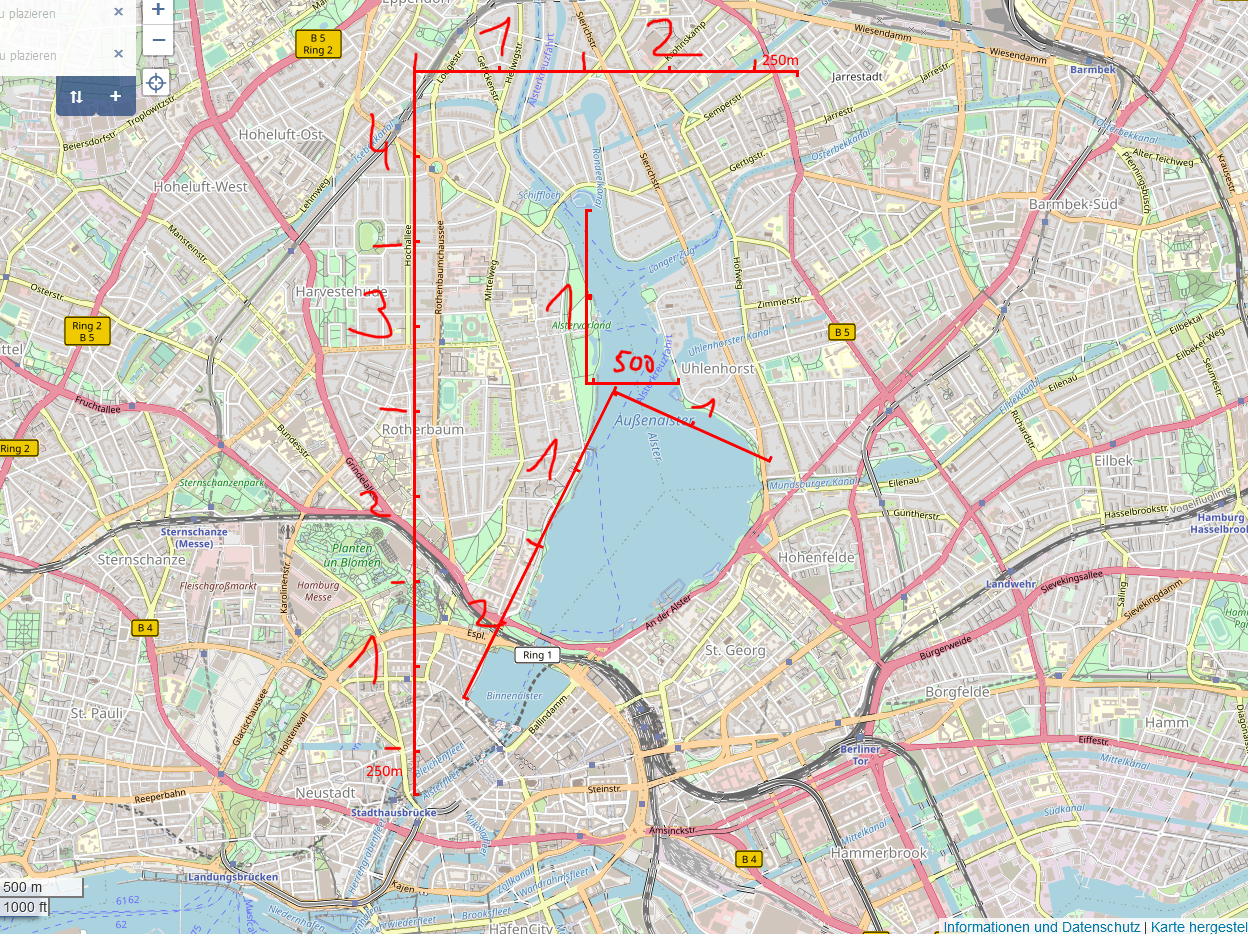
\includegraphics[width=0.75\textwidth]{calc-area}
    \caption{Grobe Flächenberechnung der bewohnbaren Bereiche}
    \label{fig:calc-area}
\end{figure}

Aus der Grafik~\ref{fig:calc-area} lassen sich folgende Flächen ablesen:

\begin{align}
    A &= (4,25~\unit{~km} * 2,25~\unit{~km}) - (0,5~\unit{~km}^2 + 2~\unit{~km}^2) \\
    &=  9,56~\unit{~km}^2 - 2,5~\unit{~km}^2 \\
    &=  7,06~\unit{~km}^2
\end{align}

Zuletzt wird noch die Multiplikation der durchschnittlichen Einwohnerdichte mit dem Flächeninhalt berechnet:

\begin{align}
    Gesamtanzahl Agenten &= 7,06~\unit{~km}^2 * ((60.541~\unit{~Einw~je~km}^2) / 8) \\
    &= 7,06~\unit{~km}^2 * (7.567,625~\unit{~Einw~je~km}^2) \\
    &= 53.427,4325~\unit{~Einw.~je~km}^2 \\
    &\approx 53.427~\unit{~Einw.~je~km}^2
\end{align}

Mit den Voraussetzungen lässt sich für jeden beliebigen Zeitpunkt an einem Arbeitstag eine Annäherung mit der Interpolationsgleichung~\ref{fig:interpolation} berechnen.
In der Simulation wird für jede Stunde, die neu angefangen wird, ein neuer Wert aus der Gleichung mit der durchschnittliche Einwohnerdichte multipliziert und damit als für diese Stunde, aktive Anzahl an Agenten festgelegt.
In dieser Simulation werden nur Daten für jede Stunde genommen, da der \code{BicycleLeader} ebenfalls nur jede Stunde einmal die Route fährt.

% The section about the agents' routes
% @author Kalvin Döge
%

\subsection{Agentenrouten}\label{subsec:routs}

In diesem Model haben \code{HumanTraveler} nur zwei Punkte auf ihrer Route, die sie erreichen müssen: Den Startpunkt, auf dem sie beginnen, und das Endziel, das ein beliebiger Punkt im Simulationsbereich ist.
Diese Agenten haben, wie bei dem Unterkapitel ,,Modalitäten`` bereits erwähnt, dafür drei verschiedene Transportarten zur Verfügung, und sind nicht weiter eingeschränkt in der Art und Weise, wie sie zum Zielpunkt gelangen.

\begin{figure}[h]
    \centering
    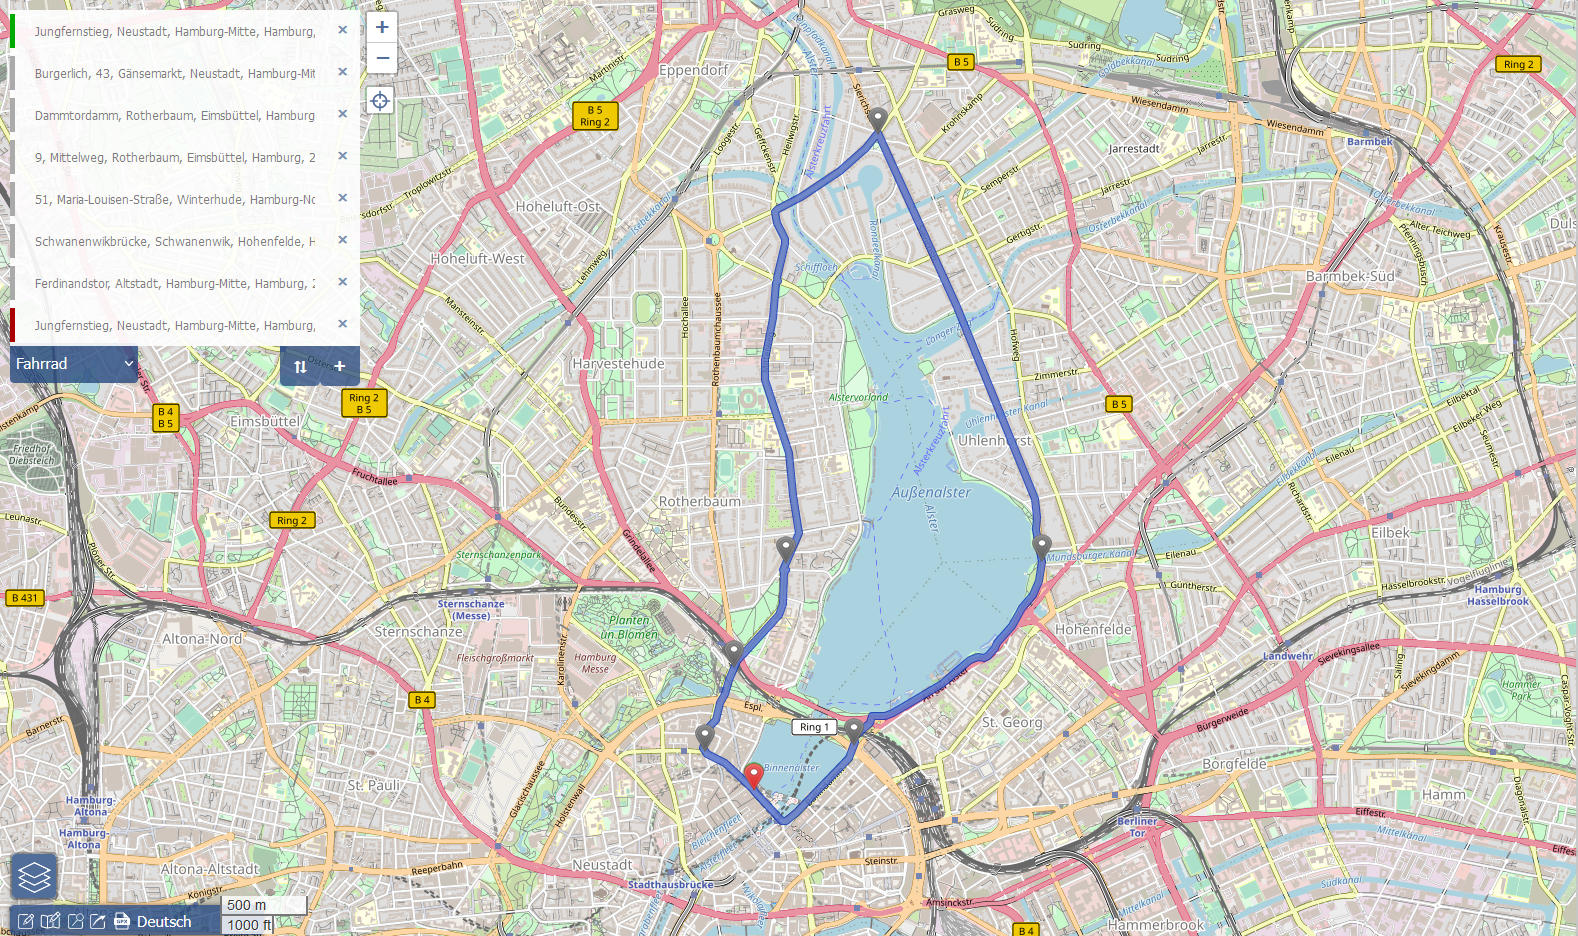
\includegraphics[width=1.00\textwidth]{route}
    \caption{Route der Bicycle-Leader mit den 8 Zwischenpunkten}
    \label{fig:bicycleleader-route}
\end{figure}

Der \code{BicycleLeader} wiederum, wie anhand der Grafik~\ref{fig:bicycleleader-route} zu entnehmen ist, hat 8 Punkte abzufahren, die um die Binnen- und Außenalster verteilt sind:
Die Route beginnt und endet bei dem Café Alex, während die restlichen 6 Punkte verteilt um die Alster platziert sind, damit eine Rundfahrt bei möglichst vielen Lichtsignalschaltungen geplant sind.



% The section about the agents of the simulation itself
% @author Kalvin Döge
%


\section{Lichtsignalschaltungen}\label{sec:lightsignals}

Die Lichtsignalschaltungen stellen die größte Barriere und der Fokus dieser Simulation: Ihre Aufgabe ist es, Pkws und Fahrräder aufzuhalten, wenn sie in der Rotphase sind und sie durchzulassen, wenn sie Grün sind.

% The section about the lightsignals' generel description
% @author Kalvin Döge
%

\subsection{Beschreibung der Lichtsignalanlagen}\label{subsec:description}

Während der Rotphase ist es möglich, dass sich mehrere Verkehrsteilnehmer an der Ampel anstauen und dadurch eine Warteschlange bilden, die sich erst bei Grün mit einer Geschwindigkeit von einem Verkehrsteilnehmer pro Sekunde leert.
Bei einer Warteschlange von 20 Leuten ist es also der letzten \code{HumanTraveler} erst möglich, die Ampel hinter sich zu lassen, sobald alle 19 Verkehrsteilnehmer vor dem \code{HumanTraveler} nach 19 Sekunden durchgelassen wurden.

Die Positionsdaten der Ampeln im Simulationsbereich sind mit dem OpenStreetMap-Tool cite{OSF2004} entnommen worden und dann für die Simulation aufbereitet in Form von \code{Longitude}- und \code{Langitude}-Werten.

% The inner workings of the light signals
% @author Kalvin Döge
%

\subsection{Funktionsweise von Lichtsignalschaltungen}\label{subsec:workings}

Die Funktionsweise der Lichtsignalschaltungen während der Simulation lässt sich in zwei Schritte zusammenfassen: 1.\ Timer fortsetzen und 2.\ die Warteschlange überprüfen.

Der Timer wird im ersten Schritt um eine Sekunde fortgesetzt.
Ist der aktuelle Timer-Wert über der Zeitgrenze von einer Rot-, Gelb- oder Grünphase, wird die Phase gewechselt.
Ist der Timer-Wert über die Summe von Rot-, Gelb- und Grünphasenlänge hinaus, setzt sich der Timer wieder zurück auf 1 verstrichene Sekunde.

Im zweiten Schritt wird die Warteschlange überprüft.
Ist der Verkehrsteilnehmer nicht mehr an dieser Ampel, weil der Teilnehmer der erste in der Schlange ist und die derzeitige Ampelphase Grün ist, so wird dieser aus der Warteschlange entfernt.
Das Wegfahren selbst unternimmt immer noch der Pkw-Fahrer selbst.

% The section about the lightsignals' phases
% @author Kalvin Döge
%


\subsection{Lichtsignalphasen}\label{subsec:phases}

Für dieses Modell wurde eine Aufnahme einer Lichtsignalschaltung getätigt, um eine Zeitangabe für die typische Rot- und Grünphasenlänge zu bekommen.
Die Stadt Hamburg hat auf Nachfrage keine Daten veröffentlichen wollen oder im Internet zur Verfügung gestellt, welche Ampeln wie lange im ,,Normalzustand`` Grün- und Rotphasen haben, also ist die Aufnahme nicht repräsentativ für alle simulierten Lichtsignalanlagen, jedoch reichen sie für das Szenario aus, das simuliert werden soll.

In der Aufnahme haben die Lichtsignalphasen folgende Längen:
\begin{itemize}
    \item Rotphase: 40 Sekunden
    \item Grünphase: 35 Sekunden
    \item Gelbphase: 1 Sekunde
\end{itemize}

Diese Zeiten dienen als Initialwerte, um danach iterativ sich dem Optimum von der Zeitschaltung zu nähern.

% The section about the lightsignals' types
% @author Kalvin Döge
%


\subsection{Lichtsignaltypen und Bezug zur Realität}\label{subsec:types}

Lichtsignalschaltungen sind in der echten Welt nicht nur mit Zeitschalter ausgestattet.
Ein Großteil derer können auch über Fernzugriffe bereits gesteuert und zu einer grünen Welle umgestellt werden.
Auf Seite 42 der Visionen von Hamburg 2030 \cite{HHH2014} aus dem Jahr 2014 wird bereits erwähnt, dass die bei Lichtsignalschaltungen eingebauten Induktionsschleifen für Busse oder bei Abbiegespuren zum Einsatz kommen, doch können auch, je nach Tageszeit, diese zur Verkehrsanpassung genutzt werden und eine ,,Grüne Welle`` für die Verkehrsteilnehmer ermöglichen.
Auch wenn die Schaltung nicht für Fahrradfahrer, sondern an erster Stelle für Pkw-Fahrer gedacht ist, so soll sich diese Simulation darauf fokussieren, für beide eine Schaltung zu finden, die sowohl Pkws als auch Fahrräder eine ,,Grüne Welle`` ermöglicht.


% The section about the project architecture, preparing the implementation
% @author Kalvin Döge
%


\section{Projektarchitektur}\label{sec:projectarchitecture}

Die Architektur dieses Modells ist wie folgt:

\begin{figure}[h]
    \centering
    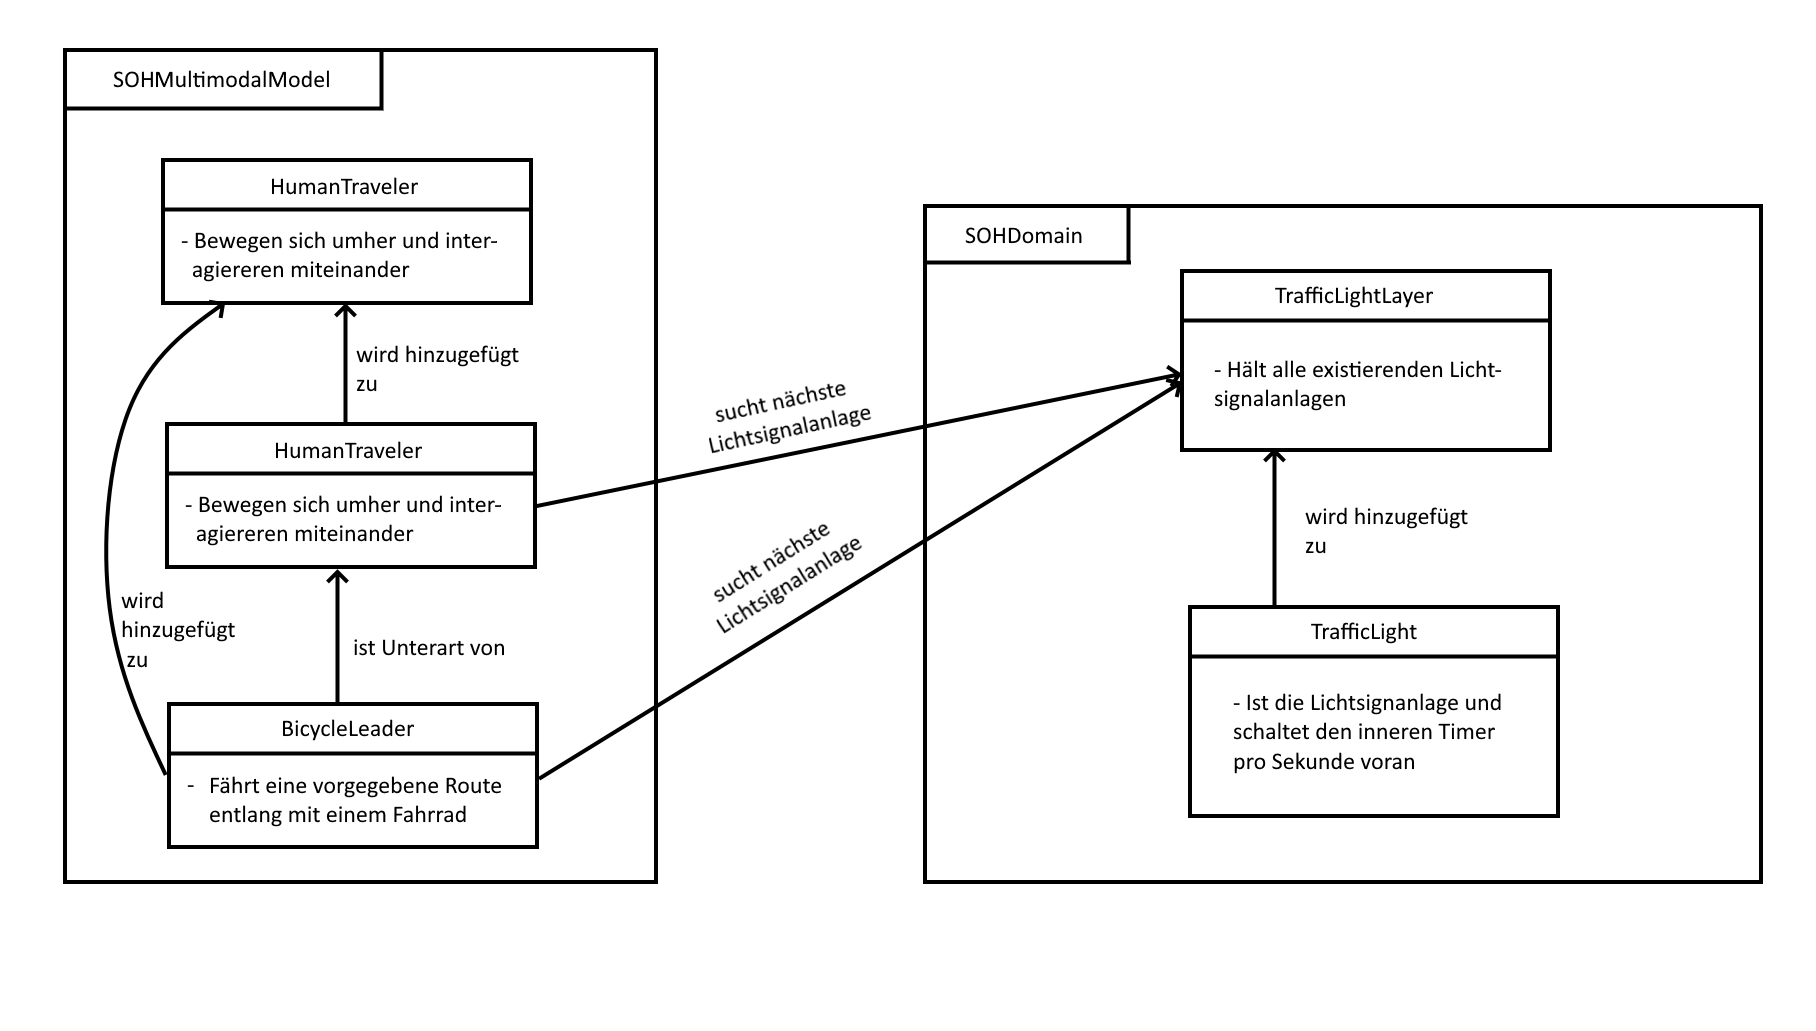
\includegraphics[width=0.75\textwidth]{architecture}
    \caption{Klassendiagramm der Agenten und Entitäten}
    \label{fig:class-diagramm}
\end{figure}

\code{HumanTraveler} werden jede Stunde erschaffen und zu ihrem \code{HumanTravelerLayer} hinzugefügt.
Die erschaffenen \code{HumanTraveler} bewegen sich auf dem \code{HumanTravelerLayer}, auf der sie mit anderen Agenten interagieren können.

Zu jeder vollen Stunde wird ein \code{BicycleLeader} in dem \code{HumanTravelerLayer} hinzugefügt und erhält dann über die \code{BicycleLeaderRoute} die zugewiesenen Routenpunkte, die dieser abfahren muss.

Die \code{TrafficLight}s werden zu Beginn vollständig in die Simulation geladen und zu einem \code{TrafficLightLayer} hinzugefügt.
Danach stehen sie jedem \code{HumanTraveler} zur Verfügung als Referenz, sobald diese wiederum erstellt werden.
\code{BicycleLeader} sind dabei eine Unterklasse der \code{HumanTraveler} und haben somit auch Zugriff auf den \code{TrafficLightLayer}.


Ein \code{TrafficLight} besitzt die folgenden Eigenschaften: Die Position angegeben als \code{Longitude} und \code{Latitude}, eine zufällig zugewiesene GUID namens ,,\code{EntityID}``, die Länge der Rot- und Grünphase als \code{LengthPhaseRed} und \code{LengthPhaseGreen}, die aktuell verstrichene, interne Zeit als \code{CurrTime}, die aktuelle Lichtsignalphase \code{CurrPhase} und zuletzt noch die wartenden Agenten über eine Warteschlange: \code{WaitingRoadUsers}.

\code{HumanTraveler}s können ein \code{Bicycle}, \code{Car} oder nichts bei sich erschaffen.
Eines dieser Modalitäten ist dann ihr Transportmittel, das \code{Vehicle}.

\code{BicycleLeader} sind identisch zu den \code{HumanTraveler}s, bis auf die Einschränkung, dass sie nur \code{Bicycle} nutzen beziehungsweise zu Fuß zum \code{Bicycle} gehen können.


\code{HumanTraveler} nutzen für das Erreichen ihres Zieles den \code{RouteFinder}, mit der sie eine Route zum Abfahren berechnet bekommen.


\code{TrafficLight}s haben folgende Funktionen, die eine Relevanz für sie selbst oder für andere Agenten in der Simulation haben:

\code{public void Tick()} setzt die innere Zeitschaltung der Ampel fort und damit auch die nächste \code{CarLightSignalPhase}, zum Beispiel von Gelb zu Rot.

\code{public void CheckQueue()} überprüft die aktuelle Warteschlange und entfernt, sobald der Agent nicht mehr warten sollte, ihn aus der Warteschlange.

\code{public Boolean Enter(IAgent IAgent)} fügt den angegebenen Agenten zur Warteschlange hinzu, sollte die aktuelle \code{CarLightSignalPhase} Rot sein.

\code{public Boolean CanPass(IAgent IAgent)} gibt einen Wahrheitswert zurück, ob der Agent sich überhaupt in der Nähe der Ampel befindet und wenn ja, ob dieser einfach vorbeifahren kann wegen eines grünen Lichtsignales und keinen wartenden, anderen Agenten.

\code{public Boolean IsQueued(IAgent IAgent)} überprüft und gibt einen Wahrheitswert zurück, ob der Agent noch in der Warteschlange notiert ist.


% The section about the projects limits
% @author Kalvin Döge
%


\section{Umfang der Arbeit}\label{sec:delimitation}

Dieser Abschnitt beschäftigt sich mit den Grenzen dieser Arbeit und Simulation.

Dadurch, dass im realen Leben Lichtsignalschaltungen verschiedenster Sicherheitsvorkehrungen unterliegen müssen, damit im Verkehr Sicherheit für alle Verkehrsteilnehmer gewährleistet werden kann, wäre eine Einbindung dieser Vorkehrungen für die Simulation ein wichtiger Realitätsaspekt.
Doch aufgrund von fehlenden Daten und genauer Auskunft der Stadt Hamburg, welche Entscheidungen Lichtsignalanlagen treffen beziehungsweise nach welchem Design sie entwickelt wurden, um die Sicherheit zu ermöglichen, fällt auch dieser Realitätsaspekt aus der Simulation aus.

Zudem werden viele Umwelteinflüsse nicht erst in der Simulation eingebaut: Beispielsweise werden Ereignisse wie Wetter, Unfälle, Baustellen oder verschiedene Verkehrsteilnehmertypen, etwa wie zu langsam Fahrende oder stetig die Spur wechselnde Teilnehmer, nicht berücksichtigt.

Die für diese Simulation genutzten Werte, wie zum Beispiel die der gesamten Agentenzahl oder die der Lichtsignalphasenlänge, sind ebenfalls aufgrund fehlender Statistiken oder Daten nicht sehr realitätsnah.
Beispielsweise wäre es angemessener, jede Lichtsignalschaltung auf der für \code{BicycleLeader} vorgesehenen Route mehrere hunderte Male zu beobachten, nur um dann eine aussagekräftigere Zeit von Rot- und Grünphasen tätigen zu können, damit statistische Abweichungen nicht potenziell das Endergebnis beeinflussen könnten.

Die Realität müsste für die Simulation über die Daten, Umwelteinflüssen und Agententypen abgebildet werden, damit ein praktischer Nutzen für die Stadt Hamburg entstehen könnte.
Entsprechend bleibt der Nutzen dieser Arbeit für die Stadt Hamburg im theoretischen Bereich.


    % The fourth chapter, about the implementation of the code
% @author Kalvin Döge
%


\chapter{Implementierung}\label{ch:implementierung}

In diesem Kapitel wird die Implementation ausgeführt, wie auf dem MARS-Framework basierend die funktionalen und nichtfunktionalen Anforderungen sowie das fachliche Datenmodell eingebaut wird.
Dazu wird auf die Ein- und Ausgabedaten und Implementationslimitationen eingegangen.

% The section about the implemented agents, entities and layers
% @author Kalvin Döge
%


\section{Agententen, Entitäten und Layer}\label{sec:agents-entities-layers}

In diesem Abschnitt wird über das Verhältnis der Agenten, Entitäten und Layer zueinander genauer eingegangen.
Alle Klassen aus der Grafik~\ref{fig:agents-entities-layer} sind gleichbedeutend vom Namen her mit den Komponenten aus dem fachlichen Datenmodell:

\begin{figure}[h]
    \centering
    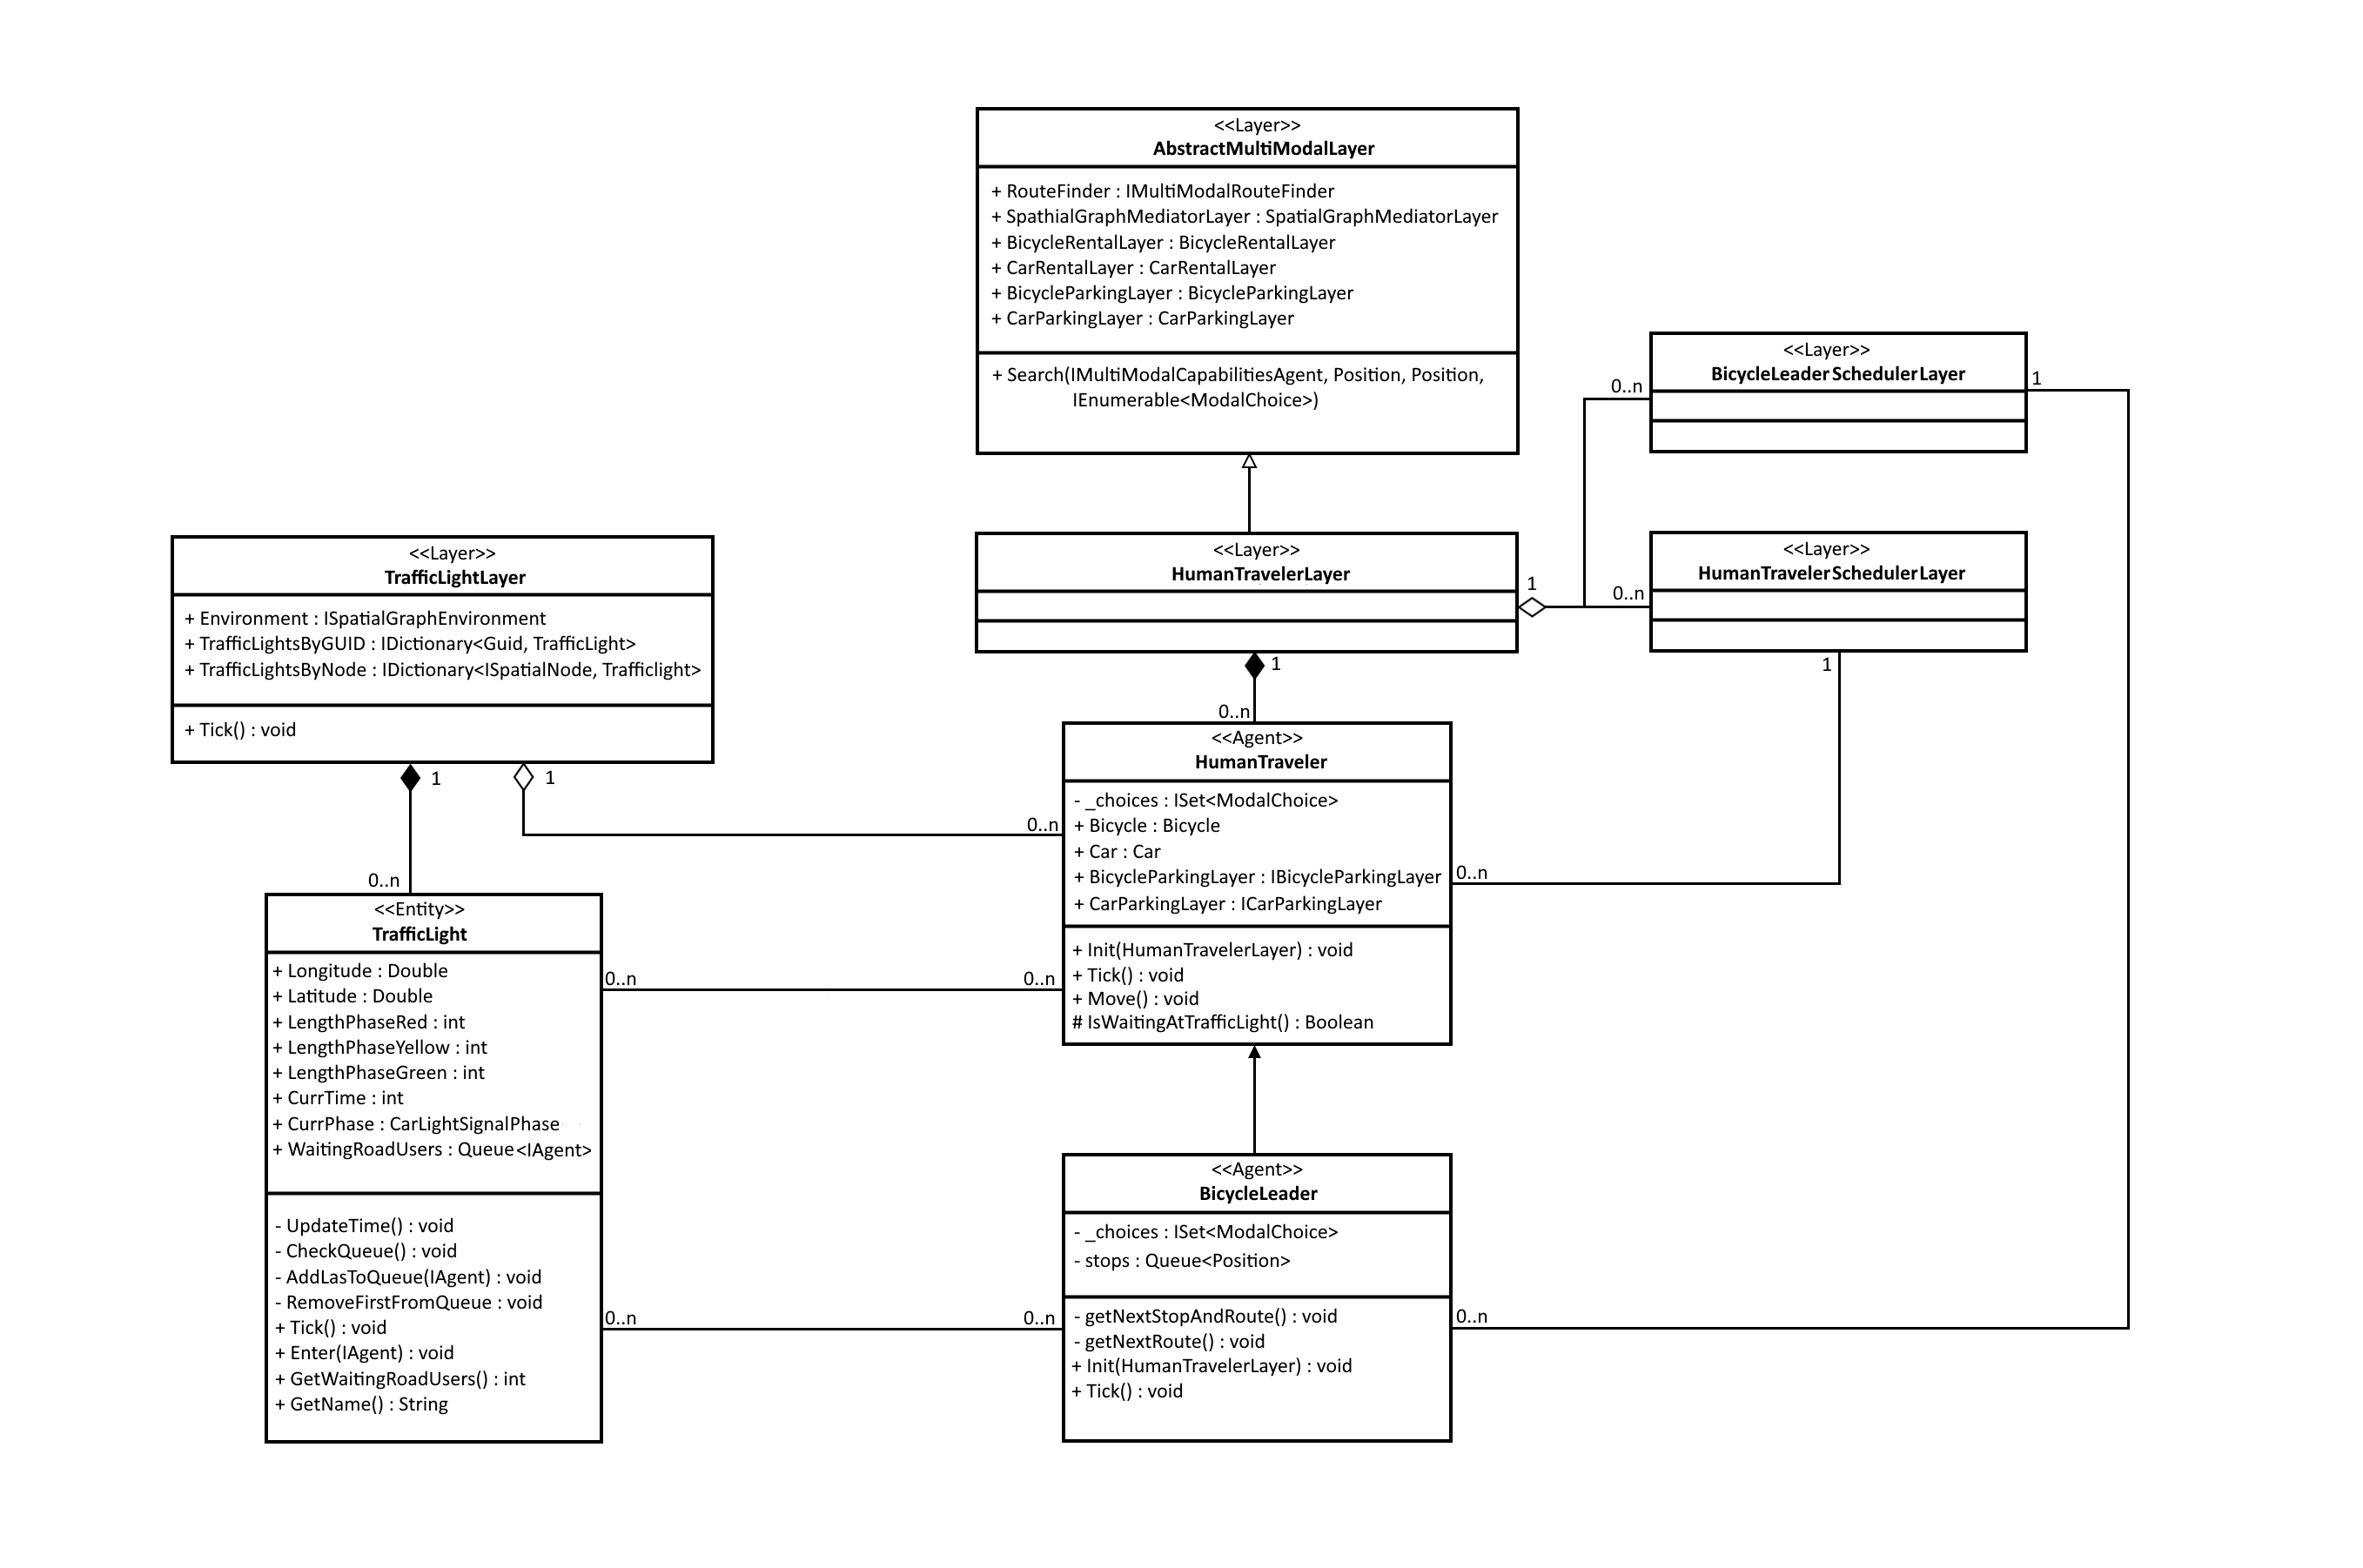
\includegraphics[width=1.00\textwidth]{agents-entities-layer}~\caption{Das technische Datenmodell aller Agenten, Entitäten und Layer}
    \label{fig:agents-entities-layer}
\end{figure}

In der Grafik~\ref{fig:agents-entities-layer} wurden einige überflüssige Eigenschaften, Methoden und Klassen weggelassen, um die Lesbarkeit und Übersichtlichkeit des Datenmodells zu erhöhen.

\textbf{Agent \code{BicycleLeader}:}
\begin{itemize}
    \item Der \code{BicycleLeader} hat Modalitäten zur Auswahl \code{\_choices}, die aber nur das Fahren eines \code{Bicycle}s, \code{RentalBicycle}s und das zu Fuß gehen über \code{WalkingShoes} erlauben.
    \item Dabei ist eine Referenz auf ein \code{Bicycle} und \code{RentalBicycle} gegeben von der geerbten Klasse \code{HumanTraveler}, die wiederum von einer Mehrzahl von Facaden erbt.
    \item Die zu fahrende Route ist beim \code{BicycleLeader} durch die Eigenschaft \code{stops} als Positions-\code{Queue} dargestellt.
    \item \code{BicycleLeader} haben zwei Funktionen zur Verfügung, um den nächsten Schritt ihrer Route zu berechnen: \code{getNextRoute()} sucht mit dem bestehenden Start- und Zielpunkt eine \code{MultimodalRoute}, während die Funktion \code{getNextStopAndRoute()} den nächsten Punkt aus der \code{stops}-Queue entnimmt, dies als das neue Ziel setzt.~Danach wird eine neue Route dorthin berechnet.
    \item Zur Routenberechnung wird der \code{RouteFinder} mit der Methode\linebreak\code{Search(MultiModalCapabilitiesAgent, Position, Position, IEnumerable<ModalChoice>)} aus dem \code{HumanTravelerLayer} aufgerufen.~Die eingegebenen Argumente meinen dabei als erstes den \code{BicycleLeader} selbst, die Startposition, die Zielposition und die dabei zur Verfügung stehenden Modalitäten des \code{BicycleLeader}s.
    \item Die Funktion \code{Tick()} setzt den nächsten Simulationsschritt des \code{BicycleLeaders} in Gang.~In dieser wird ebenfalls die vom \code{HumanTraveler} geerbte Funktion \code{Move()} ausgeführt.
    \item Die von \code{HumanTraveler} geerbte Funktion \code{IsWaitingAtTrafficLight()} wird ebenso in \code{Tick()} aufgerufen, um auf eine naheliegende \code{TrafficLight} zu prüfen: Ist ihre \code{CurrPhase} entweder \code{CarLightSignalPhase.GREEN}, also grün, oder \code{CarLightSignalPhase.YELLOW}, also gelb, so kann der \code{BicycleLeader} passieren.~Wenn nicht, hält er hier und der \code{BicycleLeader} entfernt sich über einen \code{UnregisterAgent} aus der Simulation.
    \item Hält der \code{BicycleLeader}, so gibt er dies an zusammen mit dem Standort des \code{TrafficLight}s.
\end{itemize}

\textbf{Agent \code{HumanTraveler}:}
\begin{itemize}
    \item Der \code{HumanTraveler} hat alle Modalitäten zur Auswahl: \code{Car}, \code{Bicycle}, \code{RentalCar}, \code{RentalBicycle} und \code{WalkingShoes}.
    \item Die zu fahrende Route ist beim \code{HumanTraveler} durch die Funktion \linebreak\code{Init(HumanTravelerLayer)} gegeben.~Diese ruft die \code{Init(TLayer)}-Funktion der Elternklasse \code{Traveler} auf, in der zwei zufällige Punkte aus der Start- und Zielgeometrie genommen und als Start- und Zielposition festgelegt werden.~Über ein Aufruf der \code{Tick()}-Funktion wird dann die Route berechnet zwischen den Punkten.
    \item \code{HumanTraveler} benutzen ebenfalls die \code{Search(...)}-Funktion des \code{HumanTravelerLayer}s, um die Route berechnen zu lassen.
    \item \code{Tick()} setzt auch beim \code{HumanTraveler} über den Aufruf von \code{Move()} die Bewegung fort.
    \item Der \code{HumanTraveler} prüft ebenfalls mithilfe \code{IsWaitingAtTrafficLight()} vor dem Bewegen, ob er an einer \code{TrafficLight} steht.~Wenn ja, betritt er die Warteschlange von ihr.~Wechselt die \code{TrafficLight} die \code{CurrPhase} zu \code{CarLightSignalPhase.YELLOW} oder \code{CarLightSignalPhase.GREEN}, so fährt er weiter.
\end{itemize}

\textbf{Entität \code{TrafficLight}:}
\begin{itemize}
    \item Die \code{TrafficLight} ist definiert über die Position als \code{Longitude} und \code{Latitude}, eine festgelegte \code{LengthPhaseRed}, \code{LengthPhaseYellow} und \code{LengthPhaseGreen} und hat eine zufällige Zahl zwischen einer dieser Phasen als \code{CurrTime}.~Sie ist zufällig gewählt, damit keine Synchronisation mit den anderen Ampeln vorliegt.
    \item Die \code{WaitingRoadUsers} ist die Warteschlange der wartenden Agenten.
    \item Diese wird durch die \code{CheckQueue()}-Funktion immer wieder überprüft, ob ein Agent aus der Warteschlange entfernt werden kann.~Ist die \code{CurrPhase} bei \code{GREEN} oder \code{YELLOW}, wird pro \code{Tick()}-Aufruf der vorderste der Warteschlange entfernt über die Funktion \code{RemoveFirstFromQueue()}.
    \item \code{UpdateTime()} erhöht \code{CurrTime} bei jedem Aufruf von \code{Tick()} um 1.~Ist die Summe aller drei \code{PhaseLength}s überschritten, so fängt \code{CurrTime} wieder bei 1 an.
    \item Agenten können über die Funktion \code{Enter(IAgent)} der Warteschlange beitreten, sollten sie der \code{TrafficLight} zu Nahe sein.
    \item Der Name des \code{TrafficLight}s setzt sich aus der \code{Longitude} und \code{Latitude} zusammen und wird für die Erkennung genutzt bei der Ausgabe.
\end{itemize}

\textbf{Layer \code{HumanTravelerLayer}:}
\begin{itemize}
    \item Alle \code{HumanTraveler} und \code{BicycleLeader} werden im \code{HumanTravelerLayer} festgehalten und ihre Position über den \code{SpatialGraphMediatorLayer} zusammengefasst.
    \item Der \code{HumanTravelerLayer} implementiert \code{AbstractMultiModalLayer} und stellt damit die verschiedenen Modalitäts-Layer \code{HumanTraveler}n und \code{BicycleLeader}n bereit zum Interagieren.
\end{itemize}

\textbf{Layer \code{TrafficLightLayer}:}
\begin{itemize}
    \item Alle \code{TrafficLight}s werden im \code{TrafficLightLayer} festgehalten über zwei \code{Dictionary}s:
    \begin{itemize}
        \item \code{TrafficLightsByGUID}, wenn eine \code{GUID} vorliegt und mit der die zugehörige \code{TrafficLight} entnommen werden kann
        \item \code{TrafficLightsByNode}, die über einen \code{SpatialNode}, also über \code{Longitude} und \code{Latitude}-Verortung, abgespeichert werden
    \end{itemize}
    \item Die \code{ISpatialNode}s selbst sind in der \code{Environment} vermerkt und sind befüllt mit Eingabedaten bei der Erstellung über die \code{InitLayer(LayerInitData, RegisterAgent, UnregisterAgent)}-Funktion.~Die \code{LayerInitData} stellt dabei die einzelnen Einträge aus der Konfiguration dar.
\end{itemize}

\textbf{Layer \code{BicycleLeaderSchedulerLayer}:}
\begin{itemize}
    \item Dieser \code{Layer} erhält Eingabedaten mit zeitgebunden Einträgen.~Diese Einträge werden dann über die Funktion \code{Schedule(SchedulerEntry)} der Elternklasse \code{AgentSchedulerLayer} hinzugefügt und erstellen den \code{BicycleLeader} mit den eingegebenen Eigenschaften.
    \item Der \code{BicycleLeaderSchedulerLayer} stellt damit das Factory-Pattern dar: Die Funktion \code{Schedule(SchedulerEntry)} wird mit Eingabedaten aufgerufen, um zu einem bestimmten Zeitpunkt einen \code{BicycleLeader} zu erstellen.
\end{itemize}

\textbf{Layer \code{HumanTravelerSchedulerLayer}:}
\begin{itemize}
    \item Identisch zu dem BicycleLeaderSchedulerLayer erhält dieser \code{Layer} Eingabedaten mit zeitgebunden Einträgen.~Diese Einträge werden dann über die Funktion \code{Schedule(SchedulerEntry)} der Elternklasse \code{AgentSchedulerLayer} hinzugefügt und erstellen den \code{HumanTraveler} mit den eingegebenen Eigenschaften.
    \item Der \code{HumanTravelerSchedulerLayer} stellt damit ebenso das Factory-Pattern dar: Er wird mit Eingabedaten aufgerufen, um zu einem bestimmten Zeitpunkt einen \code{HumanTraveler} zu erstellen.
\end{itemize}

% The section about the usage of the given MARS-Framework
% @author Kalvin Döge
%


\section{Anbindung an das MARS-Framework}\label{sec:mars-connection}

% The section about the used in- and outputconfiguration for the simulation
% @author Kalvin Döge
%


\section{Konfiguration der Ein- und Ausgabedaten}\label{sec:input-output-configuration}

% The section about the known limitations of implementation
% @author Kalvin Döge
%


\section{Bekannte Probleme und Einschränkungen}\label{sec:limitations}



    % The fifth chapter about the evaluation of data, output by the code
% @author Kalvin Döge
%
\chapter{Evaluation}

%\input{chapters/5-evaluation/sections/}
%\input{chapters/5-evaluation/sections/}
%\input{chapters/5-evaluation/sections/}

    % The sixth chapter, containing a summary of this paper and the outlook for future papers
% @author Kalvin Döge
%


\chapter{Zusammenfassung und Ausblick zukünftiger Forschungsarbeiten}\label{ch:summary}

Diese Arbeit beschäftigte sich mit einigen Interaktionsfacetten des Verkehrs, der Simulation innerhalb einer digitalen Zwillingsstadt und die experimentelle Bestimmung einer passenden Schaltung für Lichtsignalanlagen.
Auf dem Weg zur Lösungsentwicklung sind dabei eine Reihe von Schwierigkeiten eingetroffen und den Werdegang dieser Arbeit leider erschwerten.
Der Umgang mit diesen Problemstellen hat aber dafür immer noch zu einem Ergebnis geführt und vor allem dem Author dieser Arbeit einiges gezeigt:

Das MARS-Framework bietet geeignetes Simulationspotenzial, welches nicht nur auf SmartOpenHamburg beschränkt ist.
Dabei wurde dem Author in mehreren Wegen gezeigt, unter anderem durch die von MARS implementierte und verfügbare Skalierbarkeit des Ortes und der Agentenanzahl, die Integration von Echtzeitsensordaten und auch die stetige Erweiterung des digitalen Zwillings.
Auch wenn dabei der Erfahrungsgrad von ihm anfänglich gering war, so ist er im Nachhinein betrachtet informierter als zuvor und wäre einige Aspekte dieser Arbeit anders angegangen.

Trotz all dem ist bei dieser Arbeit gezeigt worden, dass mit den simulierten Experimenten eine allumfassende Zeitschaltung nicht der geeignete Lösungsansatz für ,,grüne Wellen`` ist, auch wenn sich eine finden ließ.
Stattdessen sollen Städte lieber in nachhaltigere, ressourcenarme Alternativen investieren, die bereits in anderen Forschungsbeiträgen als solche untersucht wurden: Erweiterungen von Fahrradwegen, Fahrradverkehr an Ampeln zu bevorzugen, Steuerung der Schaltungen durch künstliche Intelligenzen, Verleihstationen von Pkws und Fahrrädern weiter verbreiten und noch einiges mehr.

Ebenso gibt diese Arbeit einen Ausblick für zukünftige Forschung, als dass folgende Verbesserungen oder Fortsetzungen untersucht werden könnten:
An das entwickelte Modell könnten Echtzeitdaten vom Verkehr eingespeist werden, die es an manchen Lichtsignalanlagen bereits gibt.
Diese Daten umfassen manchmal nicht nur den Verkehr, sondern auch die aktuellen, technischen Daten der Lichtsignalanlagen selbst.
Damit wären akkuratere Modelle möglich und mit einer Analyse des Verhaltens bestünde die Möglichkeit, eine künstliche Intelligenz zu trainieren.
Außerdem könnten Lichtsignalanlagen selbst noch erweitert werden, denn es gibt verschiedene Ampeltypen, die im Verkehr zum Einsatz kommen.
Die Detailtiefe ließe sich dabei sogar noch mehr erweitern, wenn die Vorschriften für Lichtsignalanlagen von der Stadt Hamburg verfügbar wären.
Beispielsweise würde darunter fallen: Welche Sicherheitsvorkehrungen an Kreuzungen und welche an einfachen Straßen gelten, welche Vorkehrungen bei Rechtsabbiegern gelten, wie die Sicherheit bei Fahrradampeln gewährleistet wird und so weiter.

Das Fortsetzen der Arbeit mit diesen Aspekten könnte dem Forschungsaspekt weitere Tiefe geben, die dann entsprechend zu besseren oder mehr Erkenntnissen führen.


    \bibliography{literature}

    % Appendix
    \appendix
    % !TEX root = ../thesis.tex
% appendix example chapter
% @author Thomas Lehmann
%
\chapter{Anhang}


    \IGlossary

    \Istatement

\end{document}
